\chapter{Precision characterisation of a Feshbach Resonance}
\label{Chap_Feshbach}

% epigraph (done: 2021年8月19日13:15:22)
\setlength{\unitlength}{1pt}
\setlength{\epigraphwidth}{11.5cm}
\epigraph{In physical science a first essential step in the direction of learning any subject is to find principles of numerical reckoning and methods for practicably measuring some quality connected with it. \cite{thomson_2011}}{--- William Thomson, 1st Baron Kelvin \\ \textit{Electrical Units of Measurement (1883)}}

\section{Overview}
% Introduction and purpose (done: 2021年8月19日13:19:11)
This chapter presents our precision calibration of a Na-Rb Feshbach resonance at 347.64 G. The purpose of inserting this chapter before discussing the droplet experiment is to require a precision map of the scattering length (actually not only Na-Rb but also Na-Na and Rb-Rb) as a function of the magnetic field. This narrative order is convenient for discussing the droplet experiment; however, the research in chronological order is tortuous as described in Sec. \ref{sec:intro-overview}. I learned my lesson that one should not trust any unverified data. Previous measurements of Feshbach resonance(FR) parameters of Na and Rb, by three-body-loss (3B-loss) spectrum or associating method, both encountered intrinsic systematic errors, such as thermal averaging or shifting \cite{Bartenstein2005, Zurn2013}. Due to the 
high sensitivity of the droplet phase diagram, we need the scattering length map as accurate as possible. So, we implemented the dissociation method to refine the results of FR parameters at 347.64 G resonance. In the rest of this section, we will introduce what Feshbach resonance (FR) is, discuss the previous measurement results, and finally offer the arrangement of this chapter.

% what is a FR and why use FR (done: 2021年8月13日12:45:54)
Feshbach resonance as a powerful toolbox plays its essential role in cold atom experiments. With this nob, we can tune the interaction between atoms by applying an external field. Thus, it is used to explore the few-body (or many-body) physics and form molecules that open a new field in ultracold physics. Feshbach resonance requires two channels to couple to each other. One is the open channel (or entrance channel), with which collision can produce atoms, i.e. the energy of the collision pair is larger than the asymptotic energy of the channel. Another is the closed channel which offers bound states with the set energy instead of scattering state\cite{RevModPhys.82.1225}. When the energy of one bound state in the closed channel approaching the open channel threshold (typically set to be 0), the resonance happens. Near the resonance $B_0$, the two-body scattering length is approximate as
\begin{equation}
a(B) = a_{\rm bg}\left(1+\frac{\Delta}{B-B_0}\right),
\label{FR}
\end{equation}
where $a_{\rm bg}$ is the slowly varying background scattering length, and $\Delta$ is the resonance width. By simply scanning the magnetic field, the scattering length $a$ and thus the effective two-body contact interaction can be changed from repulsive (for $a > 0$) to attractive (for $a < 0$). The capability of manipulating the interaction strengths has been playing a vital role in the study of exotic physics such as the controlled collapse~\cite{donley2001}~or soliton formation in Bose-Einstein condensates (BEC)~\cite{Khaykovich2002,Strecker2002}, the BEC-BCS crossover in quantum-degenerate Fermi gases~\citep{PhysRevLett.92.040403,PhysRevLett.92.120403,Bartenstein2004,Bourdel2004}, and more recently the formation of dilute quantum droplets~\cite{petrov2015,ferrier2016Observation,cabrera2018quantum}. In addition, FRs are used to associate atomic pairs and form weakly bound Feshbach molecules (FMs)~\cite{Kohler2006}. Combined with a subsequent two-photon Raman process, this has led to the creation of long-sought ultracold ground-state molecules~\cite{ni2008,Takekoshi2014,Molony2014,Park2015,Guo2016,Voges2020}.

% Na-Rb FR previous measurements (done 2021年8月19日13:50:52)
The typical way of tuning the scattering length by an FR in the cold atom experiment is to control the magnetic field. When the magnetic field is tuned to the vicinity of the resonance, we have a large scattering length, thus can increase the two-body collision rate. This method enables us to enhance the three-body loss rate \cite{wang2013observation}, and by scanning the magnetic field, we can obtain a loss dip (as shown in Fig. \ref{FR_loss}). This phenomenon can be used to characterize an FR directly at first glance. By a simple Gaussian fitting to extract the peak, we obtain the resonance position. The problem of calibrating an FR by this method mainly comes from the existence of lots of Efimov states near the resonance. These three-body bound states render a severe three-body loss and then broaden or shift the measurement of resonance position \cite{RevModPhys.82.1225}. Later in 2015, \cite{wang2015formation} used the association method to calibrate the 347 G and 478 G Na-Rb FR again. However, the asymmetric associating spectrum still reveals the thermal broadening and shifting, leading to inaccuracy measurement of FR parameters \cite{Bartenstein2005, Zurn2013}.

% Show a figure for one FR loss spectrum (done 2021年8月19日13:39:31)
\begin{figure}[htb]
\begin{center}
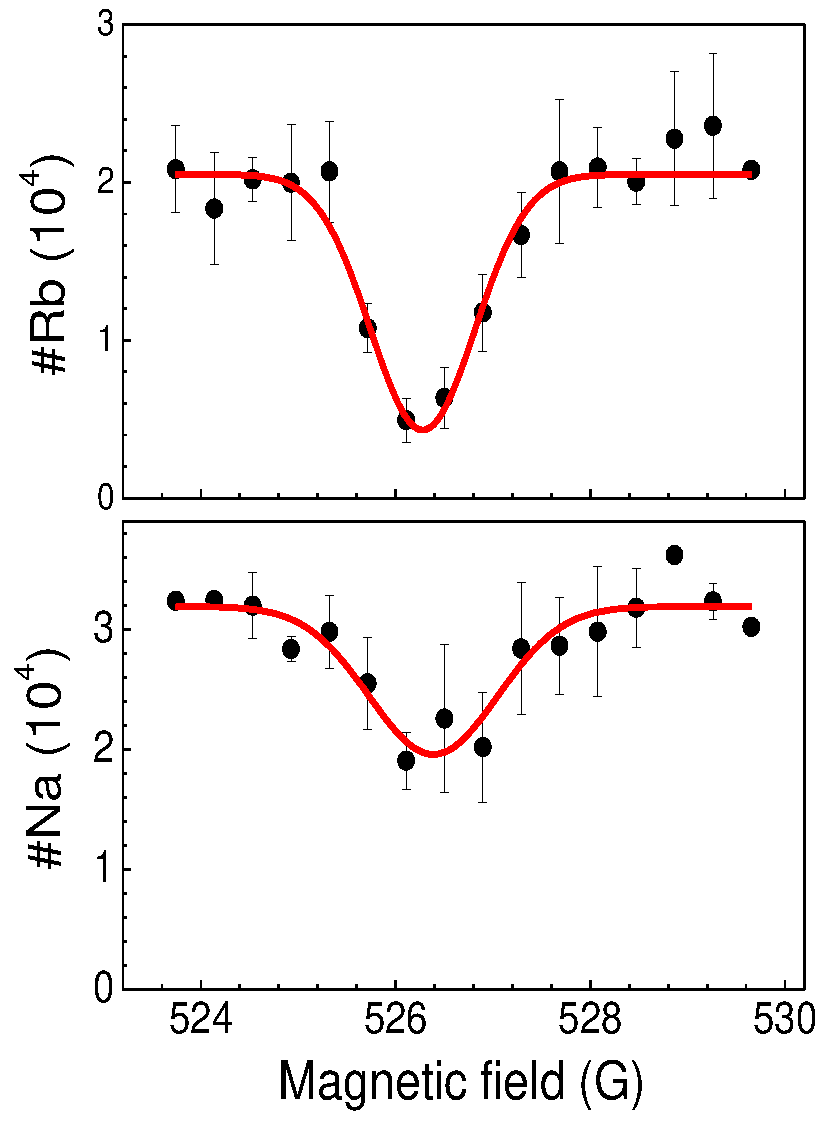
\includegraphics[width = 0.5\linewidth]{FR_loss.pdf}
\end{center}
\caption[One example of loss spectrum of Feshbach resonance.]{shows the loss spectrum of one Feshbach resonance of Na$\ket{F=1,m_F=0}$ and Rb$\ket{F=1,m_F=0}$.}
\label{FR_loss}
\end{figure}

% Introduce the dissociating method (done 2021年8月19日14:16:11)
Thus, in this Chapter, we use the most accurate method, i.e. the dissociating method, to calibrate the FR of Na and Rb at 347.64 G. To obtain an accurate map of scattering length, we need the knowledge of the molecular bound state. Recalling the discussion in chap. \ref{Chap:theory}, when we talk about quantum scattering, we typically use a pseudopotential to substitute the real complex interaction potential. However, we have to go back to the complicated real potential to obtain its scattering properties before having the scattering length. Then, an accurate map of the molecule potential is essential. Historically, people use the hot molecule to get the spectrum and then inversely deduct the potential curve \cite{}. However, this spectrum is typical only for deeply bound molecule states, which contains little information about the weakly bound states and thus the Feshbach resonances. However, our experiments need the scattering length near a Feshbach resonance, related to shallow bound states near or approaching zero when the external magnetic field is tuned across specific values. Thus, similar to the associating method, our goal is clear that we need a method to obtain these bound states energy accurately. However, to avoid the systematic error in the associating method (as shown in Fig. \ref{FR_asso}), we first form a pure molecule sample and then dissociate. Thinking in the coordinate of one molecule, one would find that this dissociation process can avoid thermal effects and thus improve the measurement accuracy. After obtaining the information of bound states, we can fit them by the coupled-channel calculation to get the Na-Rb potential. Finally, we achieve the accurate scattering length map as a function of the magnetic field. 

% Show a figure of association spectrum (done 2021年8月19日15:54:40)
\begin{figure}[htb]
\begin{center}
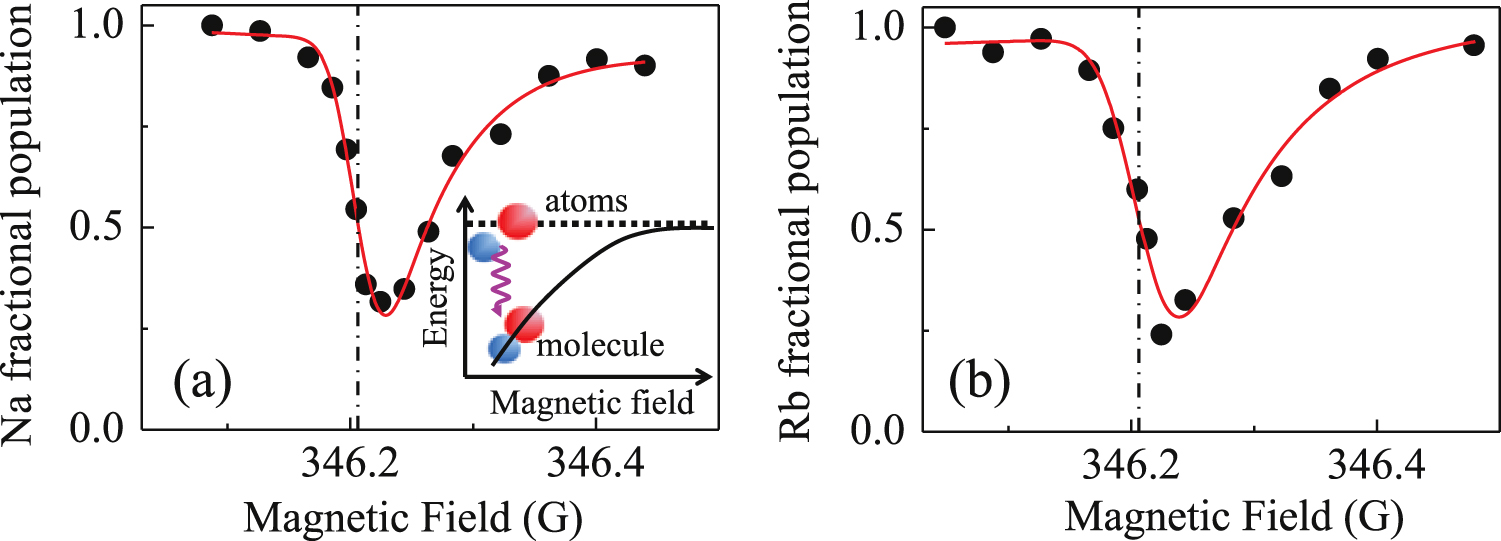
\includegraphics[width = 0.9\linewidth]{FR_asso.jpg}
\end{center}
\caption[Association spectrum of Na and Rb near 347.64 G. (Image from \cite{wang2015formation})]{Image from \cite{wang2015formation}. (a) and (b) shows the Na and Rb residue signal when doing the associating of Feshbach molecules. The dash-dot line shows the association limit, which corresponding to the zero-energy of the bound state. For a magnetic field less than the threshold, there are still association signals indicating the thermal effect. These thermal shifting and broadening smoothen the kink at the associating limit.}
\label{FR_asso}
\end{figure}

% arrangement of this chapter (done 2021年8月19日16:08:42)
The rest of this chapter is arranged as follows: Sec. \ref{sec:cali_FR} describes the method of dissociation measurement of FR molecule binding energy. Then, we apply the coupled-channel (c.c.) calculation fitting the data to obtain an accurate molecule potential curve. Finally, we achieve an accurate scattering length map. In Sec. \ref{sec:FR_spec_more}, we present ten more Feshbach resonance loss spectrums with different spin configurations of Na and Rb. They are compared to a c.c. calculation. We measured most elastic resonances and some of the inelastic, which process imaginary part of scattering length. This information can be used as a map for further exploration of a variety of Bose mixtures. Moreover, in the second part of Sec. \ref{sec:FR_spec_more} we demonstrate c.c. calculations for Rb-Rb and Na-Na both in $\ket{F=1,m_F=1}$ states. We find that the Na intraspecies interaction shows a very smooth variation from 54.5 $a_0$ (at 0 Gauss) to 64 $a_0$ (at around 900 G). This renders our estimation of Na-Na intraspecies scattering length shift about $10\%$ in the droplet paper \cite{guo2021leehuangyang}, from 54.45 $a_0$ to 60.05 $a_0$.

\section{Na-Rb Feshbach resonance at 347.64 G}
\label{sec:cali_FR}

% Method overview (done 2021年8月19日17:03:40)
This section\footnote{Announcement: most materials in this section is from our paper \cite{guo2021tunable}, which could lead to resemblance.} reports new measurements of binding energies for the state that causes the FR near 347.64 G. To reach the highest accuracy, we implement the dissociation method~\cite{Bartenstein2005,Zurn2013,Chin2005radio,Chapurin2019} to measure the binding energies. We achieve magnetic field stability at the mG level. The data are used to refine the interaction potentials for the $X^1\Sigma^+$ and $a^3\Sigma^+$ electronic states by fitting to coupled-channel bound-state calculations. We then use coupled-channel scattering calculations to obtain a highly accurate mapping $a(B)$ for the FR near 347.64~G. This has become a cornerstone for our recent experiment on the heteronuclear \Na--\Rb~quantum droplet\cite{guo2021leehuangyang}. 

% Method details (done 2021年8月19日17:27:49)
By applying a radio-frequency pulse to drive a bound-free transition~\cite{Bartenstein2005,Zurn2013,Chapurin2019}. The binding energy is obtained by subtracting the free-free transition energy from the bound-free transition energy. In the current work, as shown schematically in Fig.~\ref{FR_dis}(a), the FM lies very close in energy to the free atom pair. In this case, the dissociation can be driven by magnetic field modulation spectroscopy~\cite{Claussen2003,Thompson2005}. As illustrated in Fig.~\ref{FR_dis}(b), this is implemented by adding a small-amplitude oscillation to the magnetic field after the magnetoassociation. The oscillating magnetic field can be expressed as $B+A\times{\rm sin}(2\pi f t)$, with $B$ the final magnetic field that determines $E_{\rm b}$, and $A\ll B_0-B $. $B_0$ is the resonance magnetic field and $f$ is the modulation amplitude and frequency. Dissociation starts to occur when $f$ matches $E_{\rm b}/h$. For $f > E_{\rm b}/h$, the excess energy is converted to kinetic energy of the free atoms as $E_{\rm k} = hf - E_{\rm b}$. Due to the variation of the bound-free Franck-Condon factor with $E_{\rm k}$~\cite{Chin2005radio}, the dissociation spectrum is typically asymmetric and broad with respect to $f$.

% section outlines (done 2021年8月19日17:27:43)
In the rest part of this section, we first detailedly describe experimental measurement. Then, after obtaining the binding energies, we demonstrate the coupled-channel modelling for fitting. Finally, we compare the new calibrated parameters of Feshbach resonance at 347.64 G to the previous measurements.

% dissociation method and time sequence (done 2021年8月19日17:28:20)
\begin{figure}[htb]
\begin{center}
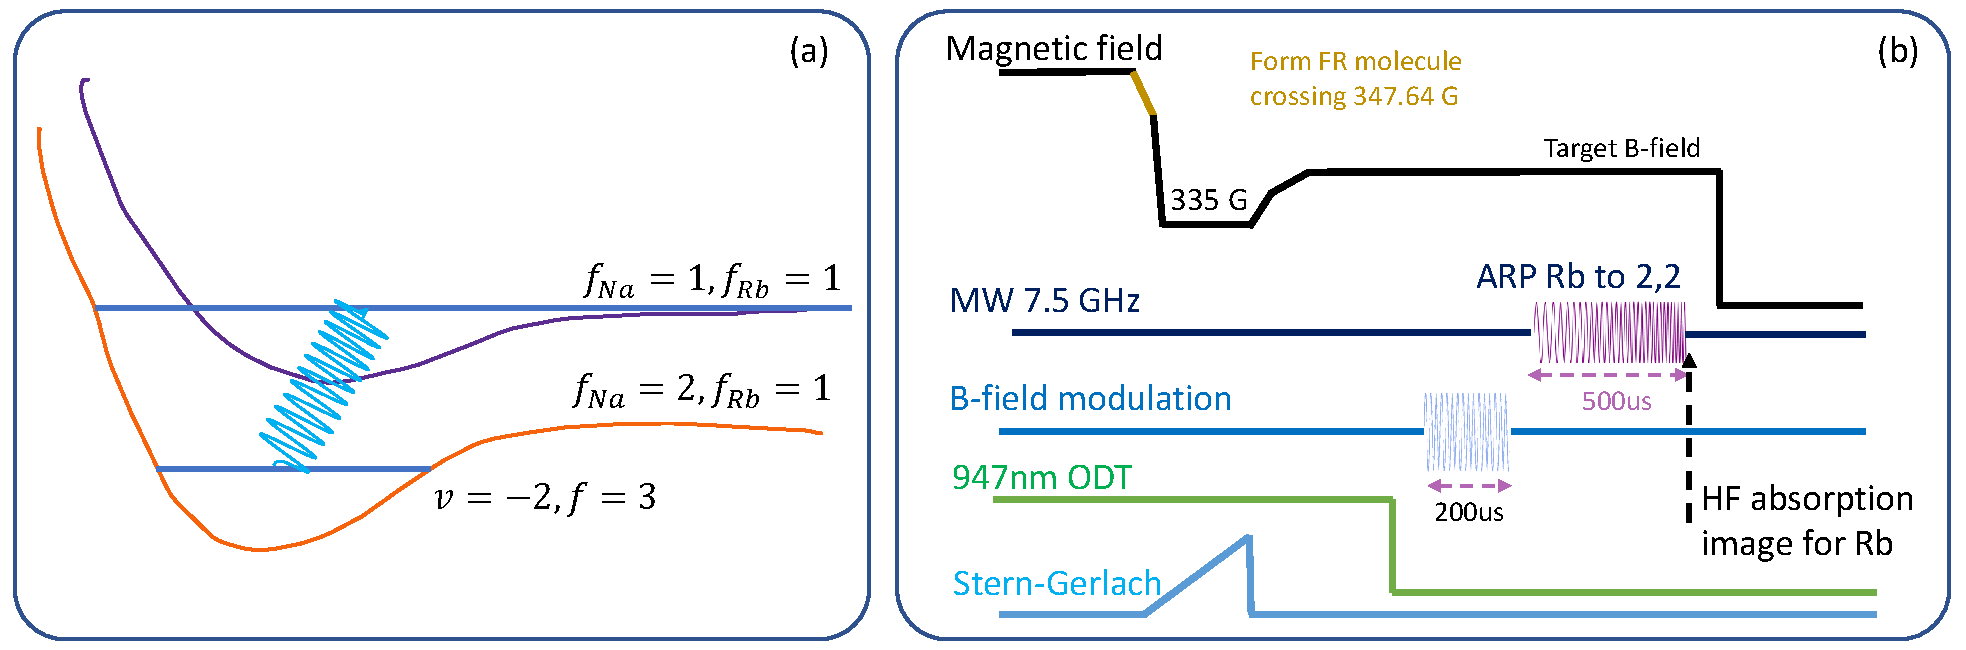
\includegraphics[width = \linewidth]{FR_dis.pdf}
\end{center}
\caption[Time sequence for measuring binding energy of Feshbach molecules]{Measuring the binding energy of a Feshbach molecule with magnetic field modulation spectroscopy. (a) The binding energy of the FM is $E_{\rm b}$. An oscillating magnetic field can drive a bound-free transition. (b) The FMs are first created by ramping the magnetic field across $B_0$. After the magnetic field is stabilized to its final value, a small-amplitude sinusoidal oscillation at frequency $f$ near $E_{\rm b}/h$ is added to dissociate the FMs and measure the binding energy. See the text for a more detailed description of the magnetic field ramping procedure.}
\label{FR_dis}
\end{figure}

\subsection{Measurement of the $^{23}$Na$^{87}$Rb Feshbach molecule binding energy}

% produce atom to molecule (done 2021年8月19日17:47:03)
Our experiment starts from an optically trapped ultracold mixture of $^{23}$Na and $^{87}$Rb atoms, both in their lowest hyperfine state $\ket{F = 1, m_F = 1}$~\cite{wang2013observation,wang2015formation,jia2020}. Magnetoassociation starts from an initial magnetic field of 350 G, just above the FR at $B_0 = 347.64$ G. The magnetic field is ramped down across the resonance to form FMs, and then to 335.6 G. At this field, the FMs have a nearly zero magnetic dipole moment; this allows us to remove the residual atoms with a short and strong magnetic field gradient without losing molecules. Afterwards, the magnetic field is ramped up to a range of target values below $B_0$ for further experiments. Following this procedure, we can routinely obtain a pure sample of \NaRb~FMs with a typical temperature of 300 nK and a trap lifetime of more than 30 ms. This short lifetime is due to near-resonance photon scattering by the 947 nm optical trap light~\cite{Guo2017,jia2020}, which is provided by a home-built diode laser system. In another experiment on \NaRb, in which a single-frequency 1064 nm laser is used as the optical trap light, FM lifetimes greater than 100 ms have been observed~\cite{Wang2019,guo2021leehuangyang}. Nevertheless, the current lifetime is more than enough for the present work, as we need only 10 ms for magnetic field stabilization and less than 1 ms for dissociation.

% remove residue atom (done 2021年8月19日21:54:33)
To obtain a high-quality dissociation spectrum, we need a pure molecule sample. If there remain atoms inside the molecule sample, though very few, because the dissociated atoms are few, it is hard to distinguish the dissociated one from the residue one. On the other hand, this part of the atom could be associated to molecules which makes the spectrum hard to subtract information. To remove residue atoms from molecules, we need to identify them by different properties, such as magnetic dipole, mass, transition frequency. To blast atoms away, we need to obtain the acceleration of atoms as large as possible and keep the molecule unaffected. The typical methods can be magnetic gradient, species-dependent optical dipole force (tune-in, tune-out trap) and resonance light for atoms. In our experiment, we originally apply the magnetic gradient at 335 G, where FMs possess zero magnetic dipoles. This method typically requires 1-2 ms to separate atoms all away from molecules, which is slow. The main limitation is the slew rate of coil current due to large coil inductance. So, later we change the method: we first transfer atoms to $\ket{F=2,m_F=2}$~state by light or by MW, then use the image cycling transition to remove the atom. With the newly upgraded full-wave loop antenna, we can achieve a high Rabi frequency for Na and Rb, both up to 50 kHz. Then, a ten us pulse could transfer all atoms to the cycling transition ground state $\ket{F=2,m_F=2}$. Then, the probe light with several saturation-intensity can blast all atoms away within less than 10 $\mu$s. More details can be found in Chap. \ref{Chap_Apparatus}.

% magnetic field modulation method (done 2021年8月19日22:07:29)
The magnetic field modulation is generated by a single loop coil driven by a low-frequency high power radio frequency amplifier. The single loop coil is placed just above the vacuum cell and coaxially with the Feshbach coils so that a modulation depth of several mG can be added to the large magnetic field. The coil has a limited modulation bandwidth of about 2 MHz. The optical trap was turned off 50 $\mu$s before applying the magnetic field modulation pulse to avoid the AC-Stark shift from the trapping light. This also reduces possible systematic errors induced by mean-field shifts of both the FMs and the free atoms as the density of FMs is lowered down. The magnetic field modulation pulse duration is chosen empirically so that the fraction of dissociation is no more than $70\%$. This is a compromise for detection signal-to-noise ratio and the requirement for using the Fermi Golden rule to fit the dissociation lineshape, which is only strictly followed for weak coupling. 

% dissociation curve 
\begin{figure}[htb]
\begin{center}
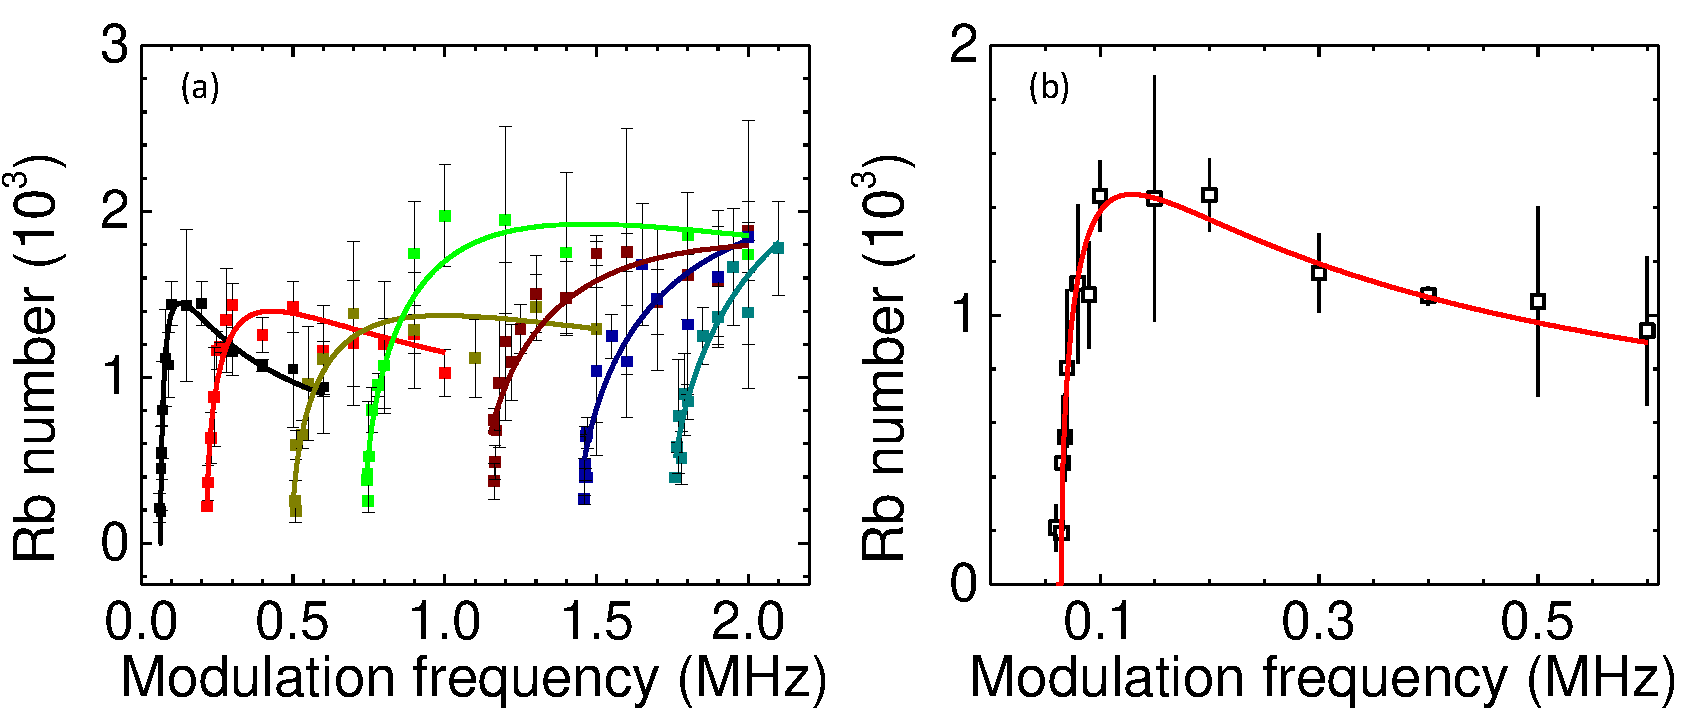
\includegraphics[width = 0.95\linewidth]{FR_spec.pdf}
\end{center}
\caption[Feshbach molecule dissociation spectrum]{Feshbach molecule dissociation spectrum at magnetic field of (a) 347.371 G, and (b) 346.000 G. The red solid curves are fitted to Eq.~\ref{eq2} to extract the FM binding energies. Because of the limited modulation bandwidth of the single-loop coil, only part of the spectrum is accessible in (b).}
\label{FR_spec}
\end{figure}

% dissociation signal (done 2021年8月21日20:22:49)
The dissociation signal is detected by absorption imaging of the fragmented \Rb atoms. Fig.~\ref{FR_spec}(a) shows several examples of dissociation spectrum versus the modulation frequency $f$ for FMs from 347.371(5) G to 345.713(5) G. Here the magnetic field is measured with radio frequency spectroscopy of the Rb atoms. Threshold behaviors are clearly visible in all dissociation spectra. Fig.~\ref{FR_spec}(b) shows the enlargement of 347.371 G dissociation spectrum in (a). There is no dissociation is observed for $f$ below 60 kHz. Since the dissociation process involves no moment transfer, the dissociation threshold is an accurate measurement of the binding energy $E_b$ of the FM. Above this threshold, the profile of the spectrum is determined by the overlap between the wave functions of the bound and free states. As the excessive energy $hf-E_b$ will be converted into the relative motion of the two atoms, the wave function of the free atoms and thus the bound-free transition rate changes with $f$. Following~\cite{Mohapatra2015}, the lineshape of magnetic field modulation spectroscopy can be represented as
\begin{equation}
N_{Rb}(f) \propto \frac{\sqrt{hf-E_b}}{hf}.
\label{eq2}
\end{equation}
From this lineshape, a dissociation maximum should be observed at $f = 2E_b/h$, afterwards, the signal will decay with a long tail following $1/\sqrt{f}$. The spectrum in Fig.~\ref{FR_spec}(b) follows this lineshape well. For the spectrum with $E_b>1$~MHz in Fig.~\ref{FR_spec}(a), the maximum is not reached due to the limited modulation bandwidth. 

% subtract kink point, i.e. the binding energy (done 2021年8月21日20:30:58)
To determine the dissociation threshold, we fit each spectrum with Eq.~\ref{eq2}. For partial dissociation spectra like Fig.~\ref{FR_spec}(b), we have verified with simulated data that $E_{\rm b}$ can still be determined with uncertainties less than 5 kHz. The variation of $E_{\rm b}$ with magnetic field, over a range from 0.061 MHz to 1.739 MHz, is plotted in Fig.~\ref{FR_bind} as black open circles. The error bar for each $E_{\rm b}$ is smaller than the symbol size. The uncertainty in the measured magnetic field is $\pm3$~mG. 

%%% Binding energy vs. Magnetic field (done 2021年8月22日11:34:39)
\begin{figure}[htbp]
\begin{center}
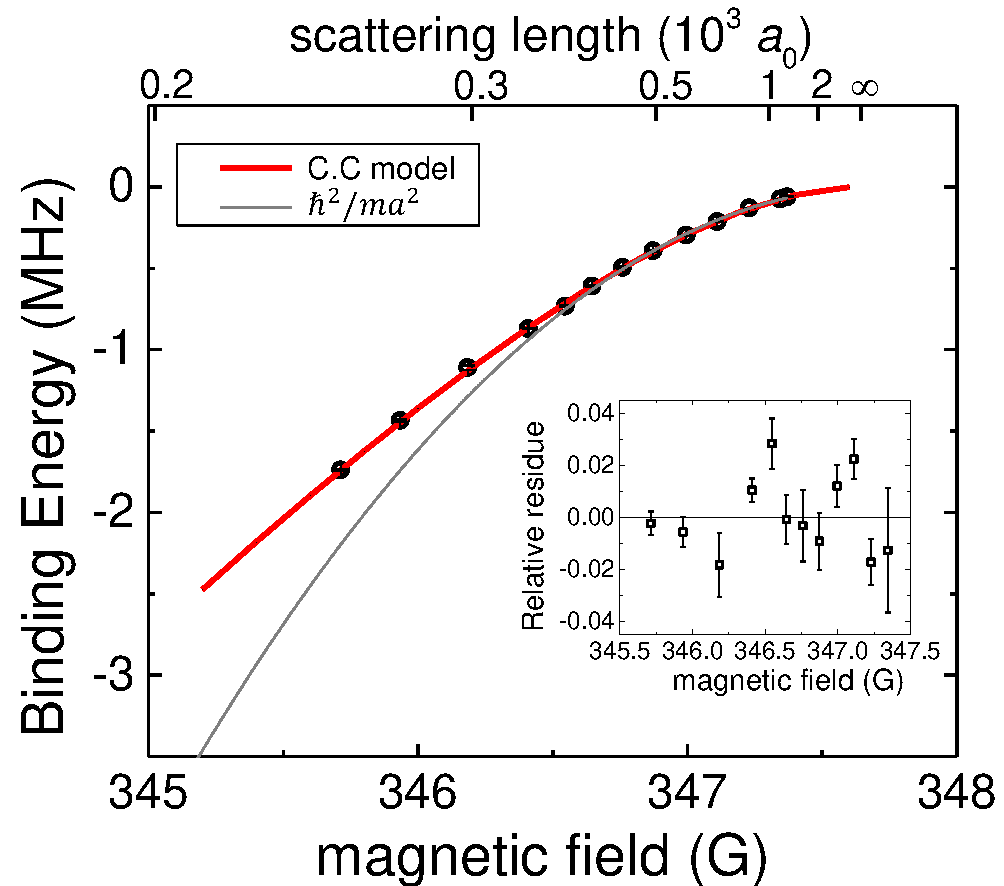
\includegraphics[width = 0.9\linewidth]{FR_bind.pdf}
\end{center}
\caption[Binding energy of $^{23}$Na$^{87}$Rb Feshbach molecules at 347.64 G]{Binding energy of $^{23}$Na$^{87}$Rb Feshbach molecules created via the FR near 347.64 G in the entrance channel Na$\ket{1,1}$+Rb$\ket{1,1}$. The black open circles are the data points measured with the dissociation method. The error bars are smaller than the symbol size. The solid red curve is from the coupled-channel (c.c.) fitting, while the thin black curve is from the universal model. Inset shows the relative residue between the experiment data and the c.c. fitting.}
\label{FR_bind}
\end{figure}

% compare association method and dissociation method (done 2021年8月22日12:05:27)
Figure~\ref{FR_asso} shows $E_{\rm b}$ for FMs that were obtained in 2015 with the association method\cite{wang2015formation} near the resonances at 347.64 G. In that work~\cite{wang2015formation}, the binding energy was fitted using the square-well model~\cite{Lange2009} with a fixed background scattering length $a_{\rm bg} = 66.77a_0$. This value of $a_{\rm bg}$ was obtained from the coupled-channel modelling of the several Feshbach resonances observed with atom-loss spectroscopy in 2013~\cite{wang2013observation}. However, the square-well model requires $a_{\rm bg}$ much larger than the interaction range, which is set by the mean scattering length of the van der Waals potential \cite{Gribakin1993}; this is $\bar{a} = 55.2\,a_0$ for $^{23}$Na$^{87}$Rb. This condition is not satisfied for the Feshbach resonances considered here. It is also well known that resonance positions measured by atom-loss spectroscopy are not accurate enough due to the complicated dynamics of three-body recombination. These issues all contribute to the inaccuracy of the Feshbach resonance parameters determined previously~\cite{wang2015formation}. In the following, we solve these issues with a new coupled-channel modelling of the binding energies of the FMs.

\subsection{Coupled-channel modeling and FR parameters}
\label{sec:cc}

% introduction about method of calibration molecular potential (done 2021年8月22日17:49:00)
After obtaining the Feshbach molecule's binding energy, we measure out how the highest shallow bound state energy varies with the magnetic field. This very shallow bound state is affected mainly by the shortest part and the long-range part ($C_6$,$C_8$,$C_{10}$) of the molecular potential curve. So, by the above measurement, we can calibrate the potential more precisely, especially at short and long-range since a typical molecular potential is achieved by the Fourier-transform molecular spectroscopy\cite{Pashov2005}, which mainly use the information for the deep binding bound state, i.e. middle range potential. We can achieve a more accurate molecular potential for Na and Rb by combining the spectroscopy data for mid-range and the measurement of shallow bound state for short and long-range. 

% what is c.c. calculation (done 2021年8月22日18:11:18)
Coupled-channel calculations rely on expanding the total wavefunction for a pair of interacting atoms in a basis set that represents the electron and nuclear spins and the relative rotation of the atoms (the partial wave $L$). Substituting this expansion into the total Schr\"odinger equation produces a set of coupled differential equations that can be solved to obtain either bound-state or scattering properties. The Hamiltonian for the interacting pair is
\begin{equation}
\label{full_H}
\hat{H} =\frac{\hbar^2}{2\mu}\left[-\frac{1}{R}\frac{d^2}{dR^2}R
+\frac{\hat{L}^2}{R^2}\right]+\hat{H}_\textrm{A}+\hat{H}_\textrm{B}+\hat{V}(R),
\end{equation}
where $R$ is the internuclear distance, $\mu$ is the reduced mass, and $\hbar$ is the reduced Planck constant. $\hat{L}$ is the two-atom rotational angular momentum operator. The single-atom Hamiltonians $\hat{H}_i$ contain the hyperfine couplings and the Zeeman interaction with the magnetic field. The interaction operator $\hat{V}(R)$ contains the two isotropic Born-Oppenheimer potentials, for the $X^1\Sigma_g^+$ singlet and $a$ $^3\Sigma_u^+$ triplet states, and anisotropic spin-dependent couplings which arise from dipole-dipole and second-order spin-orbit coupling. In the present work, scattering calculations are carried out using the MOLSCAT package
\cite{molscat:2019,mbf-github:2020} and bound-state calculations use the related packages BOUND and FIELD \cite{mbf-github:2020}. The scattering wavefunction is expanded in a fully uncoupled basis set that contains all allowed spin and rotational functions, limited by $L_{\rm max}=2$. The numerical methods are similar to those used in Ref.\ \cite{Berninger:Cs2:2013}, so will not be described in detail here.

% molecular potential structure (done 2021年8月22日18:11:15)
The interaction potential used here is based on the potential curves for the $X^1\Sigma^+$ and $a^3\Sigma^+$ states of NaRb, originally obtained by fitting to Fourier transform (FT) molecular spectroscopy~\cite{Pashov2005} and later refined by Feshbach spectroscopy with ultracold atoms~\cite{wang2013observation}. The potential curve for each electronic state, with spin $S=0$ (singlet) or 1 (triplet), has three parts: (1) a high-order power-series in the well region, which is the part best determined by FT spectroscopy; (2) a long-range extrapolation, outside internuclear distance $R_{{\rm LR},S}$, which uses theoretical dispersion coefficients and a simple exchange term; (3) a short-range extrapolation, inside $R_{{\rm SR},S}$, which uses a simple repulsion of the form $A_S + B_S/R^N_S$. $R_{{\rm SR},S}$ is usually chosen as a distance just outside the inner turning point of the potential at zero energy. For particular values of $R_{{\rm SR},S}$ and $N_S$, $A_S$ and $B_S$ are usually determined so that the short-range extrapolation has the same value and derivative at $R_{{\rm SR},S}$ as the mid-range power-series potential \footnote{This constraint was applied in the present work, but for the potential of Ref.\ \cite{wang2013observation} there are derivative discontinuities at $R_{{\rm SR},S}$.}.

% fitting to get new potential (done 2021年8月22日18:11:35)
Our goal is to adjust the interaction potential to fit the measured FM binding energies, while retaining as much as possible its ability to reproduce the FT spectra. We therefore keep the two power series that represent the singlet and triplet potential wells fixed at the fitted values of Ref.\ \cite{wang2013observation}. We also retain the long-range extrapolation in its original form, with the dispersion coefficients unchanged. We vary only the parameters $R_{{\rm SR},S}$ and $N_S$ that define the short-range extrapolations. For the triplet potential, $R_{{\rm SR},1}$ is held at its original value from Ref.\ \cite{wang2013observation}, and $N_1$ is varied; this provides sufficient flexibility to adjust the singlet scattering length and reproduce resonance positions and binding energies. For the singlet potential, however, the original value of $R_{{\rm SR},0}$ is so close to the turning point that varying $N_0$ does not allow enough change in the potential to reproduce the experimental data. In this case $N_0$ is held at its original value from Ref.\ \cite{wang2013observation}, and $R_{{\rm SR},0}$ is varied.

% add potential parameters
Here attaches the new potential parameters for Na and Rb $X^1\Sigma_g^+$ singlet and $a$ $^3\Sigma_u^+$ triplet states.
\lstset{
    backgroundcolor=\color{backcolour},   
    commentstyle=\color{codegreen},
    keywordstyle=\color{magenta},
    numberstyle=\tiny\color{codegray},
    stringstyle=\color{codepurple},
    basicstyle=\ttfamily\footnotesize,
    breakatwhitespace=false,         
    breaklines=true,                 
    captionpos=b,                    
    keepspaces=false,                 
    numbersep=5pt,                  
    showspaces=false,                
    showstringspaces=false,
    showtabs=false,                  
    tabsize=2
}
\linespread{1.0}
\begin{lstlisting}
Analytic potential energy curve for the NaRb a3Sigma+ state
(for definition of parameters see C. Samuelis et al. PRA 63, 012710 (2000)) 
-------------------------------------
Potential is given with respect to the dissociation limit which is set to 0!

For R <= 4.65 A

U(R)=A+B/R^alpha

A	-232.9656123524    cm-1
B	10710621685.47      cm-1 A^alpha 
alpha       11.492

For 4.65 < R < 11.30 A

U(R)=Sum_i[a_i*((R-R_m)/(R+b*R_m))^i]

b     -0.4700
R_m   5.60071538 A 
a_0  -203.35070852 cm-1
a_1   0.122517410860683240E+01 cm-1
a_2   0.968561681714175506E+03 cm-1
a_3  -0.167358901820848331E+03 cm-1
a_4  -0.115108986132623340E+04 cm-1 
a_5   0.538103153477437104E+03 cm-1
a_6   0.576427139041465671E+04 cm-1
a_7  -0.137759208524156093E+05 cm-1
a_8  -0.484354206699185452E+05 cm-1
a_9   0.876873287464803143E+05 cm-1
a_10  0.242372373596938676E+06 cm-1
a_11 -0.283727768851481727E+06 cm-1
a_12 -0.762367745318190078E+06 cm-1
a_13  0.433100100910781766E+06 cm-1
a_14  0.150133971696866141E+07 cm-1
a_15 -0.489081569236799405E+05 cm-1
a_16 -0.164041059210233274E+07 cm-1
a_17 -0.680259713656829204E+06 cm-1
a_18  0.665168317123337765E+06 cm-1
a_19  0.606016435356653412E+06 cm-1
a_20  0.137434664322447614E+06 cm-1
  
For R>=11.30 A

U(R)=-C_6\R^6-C_8\R^8-C_10\R^10+A_ex*R^gamma*exp(-beta*R)

C_6    0.129463596372576691E+08 cm-1 A^6
C_8    0.358980000000000000E+09 cm-1 A^8
C_10   0.130601455102733498E+11 cm-1 A^10
A_ex   0.31859846D+05 cm-1 A^(-gamma)
gamma  5.00810   
beta   2.20850 A^-1

--------------------------------
Analytic potential energy curve for the NaRb X1Sigma+ state
(for definition of parameters see C. Samuelis et al. PRA 63, 012710 (2000) 
--------------------------------
Potential is given with respect to the dissociation limit which is set to 0!

For R <= 2.7256 A

U(R)=A+B/R^alpha

A           -8490.090071421    cm-1
B           450828.6299011      cm-1 A^alpha 
alpha   4.06143861049682720

For 2.7256 < R < 11.30 A

U(R)=Sum_i[a_i*((R-R_m)/(R+b*R_m))^i]

b     -0.2100
R_m    3.64340736 A
a_0   -5030.50869783 cm-1
a_1   -0.662030723944292271E-01 cm-1
a_2    0.253807725995464061E+05 cm-1
a_3    0.929104757521979809E+04 cm-1
a_4   -0.211814748606123285E+05 cm-1
a_5   -0.284181834656136671E+05 cm-1
a_6    0.210407753693068798E+04 cm-1
a_7   -0.851968733976350748E+06 cm-1
a_8   -0.123216494098773529E+07 cm-1
a_9    0.383640579108661637E+08 cm-1
a_10   0.109125343263982777E+08 cm-1
a_11  -0.109331126199059677E+10 cm-1
a_12   0.540863749615297675E+09 cm-1
a_13   0.203930014933835602E+11 cm-1
a_14  -0.222458146577416687E+11 cm-1
a_15  -0.258727375257563232E+12 cm-1
a_16   0.419458345047378906E+12 cm-1
a_17   0.226157469213112939E+13 cm-1
a_18  -0.493156268638760059E+13 cm-1
a_19  -0.133732693094783848E+14 cm-1
a_20   0.391427433409150078E+14 cm-1
a_21   0.491914424477468672E+14 cm-1
a_22  -0.214673998282790187E+15 cm-1
a_23  -0.736821254504513125E+14 cm-1
a_24   0.806693583557253000E+15 cm-1
a_25  -0.249784752437157937E+15 cm-1
a_26  -0.198517974510287375E+16 cm-1
a_27   0.172480088271182725E+16 cm-1
a_28   0.281094984850021900E+16 cm-1
a_29  -0.441448085841028300E+16 cm-1
a_30  -0.122221795646213325E+16 cm-1
a_31   0.552071157529799900E+16 cm-1
a_32  -0.210051881065563800E+16 cm-1
a_33  -0.244906408631624500E+16 cm-1
a_34   0.238499017935224850E+16 cm-1
a_35  -0.611040299017092875E+15 cm-1

For R>=11.30 A

U(R)=-C_6\R^6-C_8\R^8-C_10\R^10-A_ex*R^gamma*exp(-beta*R)

C_6    0.129463596372576691E+08 cm-1 A^6
C_8    0.358980000000000000E+09 cm-1 A^8
C_10   0.130601455102733498E+11 cm-1 A^10
A_ex   0.31859846E+05 cm-1 A^(-gamma)
gamma  5.00810   
beta   2.20850 A^-1
\end{lstlisting}

% continuing (done 2021年8月22日18:12:09)
The shape of the curve of $E_{\rm b}$ as a function of $B$ is quite insensitive to variations in the singlet and triplet scattering lengths, represented by $R_{{\rm SR},0}$ and $N_1$. It is therefore sufficient to fit to one binding energy from each FR. For the resonance near 347.64 G, we choose the point with $E_{\rm b}/h = 0.611(6)$~MHz at 346.646(5) G, while for the resonance near 478.7 G, we choose the point with $E_{\rm b}/h = 0.400$~MHz at 478.052(10) G. The parameters $R_{{\rm SR},0}$ and $N_1$ are then adjusted so that these binding energies are reproduced essentially exactly. The resulting values are $R_{{\rm SR},0}=2.7256$~\AA\ and $N_1=11.492$. The singlet and triplet scattering lengths calculated from the fitted potentials are  $a_{\rm s} = 106.474 a_0$ and $a_{\rm t} = 68.864 a_0$, respectively. These are $0.27 a_0$ smaller and $0.24 a_0$ larger than the values of Ref.\ \cite{wang2013observation}, indicating that the triplet potential needs to be slightly more repulsive than the original at short range, while the singlet potential needs to be slightly less repulsive.

% obtain FR parameters (done 2021-8-22 18:12:32)
We use the fitted potentials to calculate the $s$-wave scattering length $a(B)$. We find that each resonance is well represented by Eq.~\ref{FR}. The parameters $B_{0}$, $\Delta$ and $a_{\rm bg}$ are obtained as described by Frye and Hutson \cite{Frye2017}, and are given in Table~\ref{tab1}. In Fig.~\ref{FR_bind}, the binding energies calculated from the universal model $E_{\rm b} = \hbar^2/2\mu a(B)^2$ using the new $a(B)$ is also shown. Compared with the coupled channel results (red solid curve), this reproduces the data only for $E_{\rm b}< 0.6$ MHz. 

% Parameters of the two low-field $s$-wave Feshbach resonances (done 2021年8月19日22:40:53)
\begin{table}[htb]
\caption{Parameters of the two low-field $s$-wave Feshbach resonances for the entrance channel Na$\ket{1,1}$+Rb$\ket{1,1}$.}
\label{tab1}\centering
\begin{tabular}{ c | c | c | c }
\hline\hline
$B_0$ (G) & $\Delta$ (G) & $a_{\rm bg}$ ($a_0$) & reference\\
\hline
347.648 & 4.255  & 76.33 & this work\\
347.64 & 5.20  & 66.77 & \cite{wang2015formation}\\
347.75 & 4.89  & 66.77 & \cite{wang2013observation}\\
\hline
478.714 & 3.491  & 71.55 & this work\\
478.83 & 4.81  & 66.77 & \cite{wang2015formation}\\
478.79 & 3.80  & 66.77 & \cite{wang2013observation}\\
\hline \hline
\end{tabular}
\end{table}

% comparison(done 2021-8-22 18:18:23)
In the present fit, the resonance near 347.64 G has shifted by about 0.08 G compared to Ref.\ \cite{wang2013observation}. The resonance near 487.7 G has shifted by more than 0.1 G. These shifts produce substantial changes in the calculated scattering lengths. Moreover, in Ref.\ \cite{wang2013observation}, the calculated scattering length was fitted using the formula
\begin{equation}
a(B)=a_{\rm bg} \left[1 + \frac{\Delta_0}{B-B_0} + \frac{\Delta_1}{B-B_1} + \dots\right],
\label{eq:FRsum}
\end{equation}
with a single $B$-independent background scattering length $a_{\rm bg}$ for all resonances. This formula breaks down when the background scattering length varies significantly between resonances. In the present work, Eq.~\ref{FR} is found to be a good local representation for each resonance, but significantly different values of $a_{\rm bg}$ are needed for the resonances at 347.64 G and 487.7 G. Such behavior can arise from many sources, including the changing spin character of atomic states with magnetic field and the presence of additional resonances not included in the summation of Eq.\ \ref{eq:FRsum}. As shown in Fig.~\ref{FR_para}, for the resonance near 347.64 G, the scattering lengths calculated with the new potential differ by about $20a_0$ from those of Ref.\ \cite{wang2015formation} in the region from 349.8 G to 350.0 G that is important for studies of Na-Rb quantum droplets. This change is significant and largely explains the discrepancies initially observed between experiment and theory in Ref.\ \cite{guo2021leehuangyang}.



%%% Binding energy vs. Magnetic field (done 2021年8月22日18:18:11)
\begin{figure}[htbp]
\begin{center}
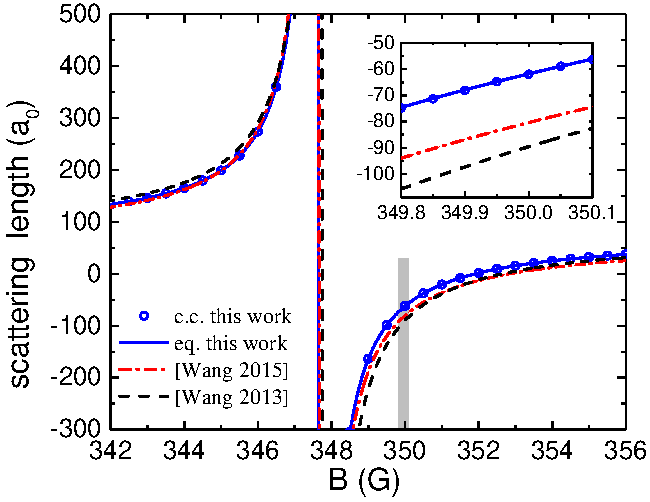
\includegraphics[width = 0.9\linewidth]{FR_para.pdf}
\end{center}
\caption[Scattering length as function of magnetic field]{Comparison of the mapping between magnetic field and scattering length with Feshbach resonance parameters obtained in this work, using coupled-channel results directly (blue open circles) and fitted to Eq.~\ref{FR} (blue solid curve) and , and in Ref.~\cite{wang2015formation} (red dash-dotted curve) and Ref.~\cite{wang2013observation} (black dashed curve), both using Eq.~\ref{eq:FRsum}. The region of interest for the droplet experiment~\cite{guo2021leehuangyang}, marked with a vertical gray bar, is enlarged in the inset. }
\label{FR_para}
\end{figure}

% some explanation for c.c. (done 2021年8月22日18:18:55)
All the coupled-channel calculations use a basis set that includes functions for partial waves $L = 0$ and $L =2$, with the effective dipolar coupling function of Ref.\ \cite{wang2013observation} unchanged. Omitting the $L = 2$ basis functions causes shifts that are on the same level as the experimental uncertainties: the calculated resonance positions and binding-energy curves shift down by between 3 and 4 mG. It is possible to include additional partial waves, but we expect the shifts to be very small. In contrast to Ref.\ \cite{wang2013observation}, we do not include any variation of the atomic hyperfine coupling with internuclear distance.


\section{Na-Rb, Na-Na and Rb-Rb scattering length summery}
\label{sec:FR_spec_more}
% overview (done 2021-8-22 18:37:21)
Besides the Feshbach resonance at 347.64 G, different combinations of the spin state of Na and Rb possess plenty of FRs. Ref.~\cite{wang2013observation} investigated the entrance channels $\ket{m_F=1}+\ket{m_F=1}$ and $\ket{m_F=-1}+\ket{m_F=-1}$ and in total observed three $s$-wave and two $p$-wave FRs. In addition, ten more $s$-wave FRs were predicted for collisions between pairs of atoms in different $F = 1$ hyperfine Zeeman states. In this section, we report the experimental observation of several of these FRs below 1000 G in 5 hyperfine Zeeman combinations. We believe these FRs will find important applications in the future, for example, in the investigation of BEC mixtures and quantum droplets with more than two components~\cite{ma2021}. 

% some words on the Na-Na scattering length (done)
With the powerful tool, MOLSCAT \cite{molscat:2019,mbf-github:2020}, we can get more precise maps of scattering length and magnetic field. Since even the background scattering length varies when the external field changes, the value of the scattering length, especially for a finite (not low) field, should be treated with more care. Here we find that the Na-Na 1,1 state have a smoothly varying background scattering length from low field to around 900 G (near the FR). Its value starts from 54.45 $a_0$ to about 64 $a_0$. For our droplet experiment, under about 350 G magnetic field, the Na-Na scattering length is 60.05 $a_0$ which is larger about 10\% than at low field.

\subsection{Na-Rb scattering length for different spin combination}

% experiment preparation state (done 2021-8-22 18:52:27)
For simplicity, we will denote the collision channel of a pair of \Na + \Rb atoms by $\ket{m_F^{\rm Na}}+\ket{m_F^{\rm Rb}}$. In ref.~\cite{wang2013observation}, both the $\ket{1}+\ket{1}$ and the $\ket{-1}+\ket{-1}$ channels were investigated and in total 3 $s$-wave and 2 $p$-wave FRs were observed. As shown in Fig. \ref{FR_more}, we detect more FRs in different combinations. The experiment for this section starts from optically trapped thermal mixtures of \Na and \Rb both in the $\ket{-1}+\ket{-1}$ channel. The number of atoms for both species are typically around $10^5$ and the sample temperatures are about 1~$\mu$K. The atoms are then transferred to selected hyperfine Zeeman levels with radio frequency (rf) rapid adiabatic passages. For each species, the $\ket{-1}\rightarrow \ket{0}$ and the $\ket{0}\rightarrow \ket{1}$ Zeeman splittings are very similar. In addition, these splittings in different species are also very similar to each other. To avoid cascade transitions and to realize species-selective state control, the state transfers are performed at 100 G where the transitions are all different by more than 500 kHz. With this method, we are able to prepare the Na-Rb mixture in all the 9 possible $m_F$ combinations of their $F = 1$ states. Then, we ramp the magnetic field to different values and hold the samples for 50 ms before releasing the atoms from the optical trap and measuring the remained numbers of atoms. Intersperses FRs manifest as losses of atoms in both \Na~and \Rb~atoms as a result of enhanced interspecies three-body recombination rates. As presented in Fig.~\ref{FR_more}, guided by the predictions in~\cite{wang2013observation}, we observe 10 FRs in 6 hyperfine Zeeman combinations. 

%%% figure of 10 more FR spectroscopy (done 2021年8月22日18:52:16)
\begin{figure}[htb]
\begin{center}
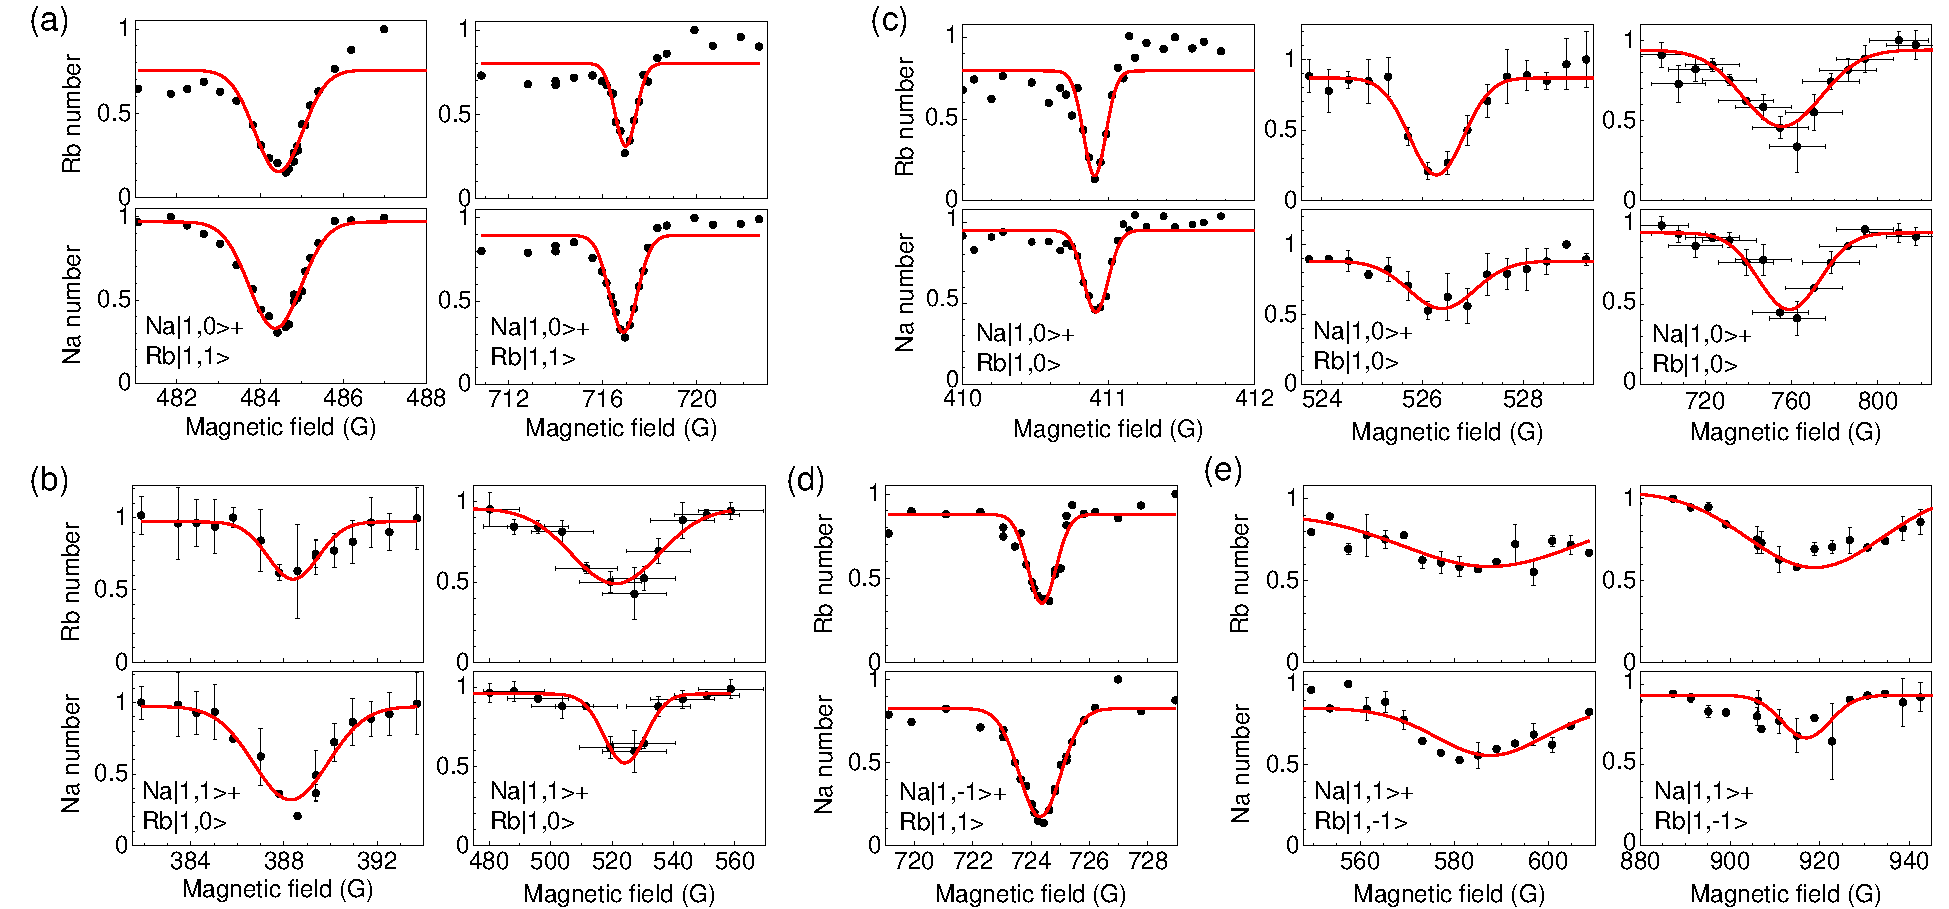
\includegraphics[width = \linewidth]{FR_more.pdf}
\end{center}
\caption[Loss spectroscopy of Feshbach resonance with different spin combinations]{Feshbach resonances in \Na-\Rb, observed by losses for atoms in the $F = 1$ hyperfine states. (a) and (b) are for the two channels in the $M_F = 1$ manifold; (c), (d) and (e) are for the three channels in the $M_F = 0$ manifold. The typical holding time at each magnetic field is 50 ms. The solid curves are from Gaussian fitting to determine the lineshape center. Error bars for the atom numbers represent one standard deviation. The large error bars for the magnetic field for the several broad loss spectra are due to less precise magnetic field control in these cases (see text).}
\label{FR_more}
\end{figure}

% implement c.c. calculation (done 2021年8月23日10:09:31)
We have carried out coupled-channel calculations of resonance parameters for both elastic and decayed resonances, using the interaction potentials obtained in Sec.~\ref{sec:cc}. The results are included in Table~\ref{fst}. For elastic resonances, the resonance positions for the lowest threshold of each $M_F$ is first located with the FIELD program~\cite{mbf-github:2020}. The FRs are then characterized using the MOLSCAT program~\cite{molscat:2019,mbf-github:2020} following the elastic procedure of Ref.~\cite{Frye2017}, which converges on the resonance position $B_0^{\rm cc}$, the elastic resonance width $\Delta$, and the background scattering length $a_{\rm bg}$. Here $a_{\rm bg}$ is a local background scattering length that is different for each resonances. In the current calculation, we have not included the spin-spin interaction, so that both the quantum number $L$ of the partial wave and its projection $M_L$ are conserved in the calculation. Since $M_{\rm tot} = m_F^{\rm Na}+m_F^{\rm Rb} + M_L$ is conserved, only closed channels with $M_F = m_F^{\rm Na}+m_F^{\rm Rb}$ the same as the colliding atoms can cause FRs.

% FR spectroscopy and c.c. calculation table (done 2021年8月23日10:11:19)
\begin{sidewaystable}[thp]
\caption[Summary table of Na-Rb Feshbach resonances with different spin combinations]{Comparison of experimental resonance positions $B_0^{\rm exp}$ with theoretical parameters for interspecies FRs below 1000 G in \Na--\Rb, for the nine $F = 1$ entrance channels. $L$ indicates the partial wave of the entrance channel. $B_0^{\rm exp}$ is the mean of the centers of the loss spectra for \Na\ and \Rb in Fig.~\ref{FR_more}, determined by Gaussian fitting. Error bars represent one standard deviation. The theoretical values are from coupled-channel calculations using the singlet and triplet potential-energy curves described in Sec.~\ref{sec:cc} with the latest potential parameters. $B_0^{\rm cc}$, $\Delta$, and $a_{\rm bg}$ are the theoretical position, elastic width, and background scattering length, respectively. The last column ``inel.?'' indicates whether the FR is subject to inelastic losses from spin exchange. For decayed FRs with inelastic losses, the resonant scattering length $a_{\rm res}$ and the inelastic width $\Gamma_{\rm inel}$ are also listed.}
\label{fst}\centering
\begin{tabular}{l|c|l|c|c|c|c|c|c}
\hline\hline
Entrance channel 				& $L$ & $B_0^{\rm exp}$(G)	& $B_0^{\rm cc}$(G)	& $\Delta$(G)	& $a_{\rm bg}$($a_0$) & $a_{\rm res}$($a_0$) & $\Gamma_{\rm inel}$(G)	& inel.? \\
\hline
Na$\ket{1,1}$ + Rb$\ket{1,1}$   & 1 	& 284.1(3)        	& 283.894			&   						 &   		& & & N     \\
						    	& 1    	& 284.2(3)         	& 283.936 			& 	&       							 & & & N     \\
    							& 1    	& 284.9(3)         	& 284.735 			&   &         							 & & & N     \\
    							& 1    	& 285.1(3)          & 284.993 			&   &         							 & & & N     \\
								& 0    	& 347.61(2)       	& 347.645 			& 4.258  			 & 76.328  	& & & N     \\
					        	& 0 	& 478.82(3)        	& 478.712 			& 3.495  			 & 71.548   & & & N     \\ \hline
Na$\ket{1,1}$ + Rb$\ket{1,0}$   & 0    	& 388.5(2)          & 388.577 			& 5.684  & 78.441                 &6548.8 & $-0.13617$& Y     \\
								& 0    	& 522(10)           & 524.286 			& 1.010  & 74.332                 & 12.906& $-11.634$& Y     \\ \hline
Na$\ket{1,0}$ + Rb$\ket{1,1}$   & 0   	&  	--		        & 358.078 			& <0.001  & 80.108                & & & N     \\
								& 0   	& 484.45(5)         & 484.569 			& 4.476  & 77.258                 & & & N     \\
								& 0		& 	--				& 570.441			& <0.001	& 73.784			 & & & N \\
								& 0   	& 716.97(6)         & 717.166 			& 5.593  & 72.998                 & & & N     \\  \hline
Na$\ket{1,1}$ + Rb$\ket{1,-1}$ 	& 0    	& 587(3)         & 580.686 			& 0.241  & $82.389 - 0.0072 i $  & $2.3917 + 0.87566 i$&$-16.596$& Y     \\
							  	& 0    	& 920(1)         & 913.431 			& 0.091  & $81.139 + 0.0352 i$ & $0.47768 + 0.12885 i$& $-30.861$& Y     \\ \hline
Na$\ket{1,0}$ + Rb$\ket{1,0}$  	& 0    	& 410.90(1)         & 409.810 			& 0.176  & 82.328                 & & & N     \\
    							& 0    	& 526.29(3)         & 526.548 			& 5.676  & 78.132                 &23515 &$-0.03772$ & Y     \\
    							& 0    	& 759(13)           & 768.781 			& 1.638  & 75.495                 &19.983 &$-12.373$ & Y     \\ \hline
Na$\ket{1,-1}$ + Rb$\ket{1,1}$ 	& 0    	& --		        & 419.648 			& <0.001  & 80.109                &0.25533 &$-0.34477$ & Y     \\
								& 0    	& --        		& 516.986 			& 0.003  & 79.401                 & & & N     \\	
								& 0    	& 724.38(4)         & 727.270 			& 4.870  & 76.444                 & & & N     \\ \hline
Na$\ket{1,0}$ + Rb$\ket{1,-1}$  & 0    	& --          		& -- 			& -- & --                             & & & N     \\ \hline
Na$\ket{1,-1}$ + Rb$\ket{1,0}$  & 0    	& --          		& 609.754 			& 0.416 & 80.572                  & & & N     \\
								& 0		& --				& 759.441			& 5.676 & 78.826				  & & & N \\ \hline	
Na$\ket{1,-1}$ + Rb$\ket{1,-1}$ & 0    	& 899.8(3)          & 900.317 			& -0.315 & 79.270                 & & & N     \\
								& 1    	& 954.2(3)          & 954.755 			&   &         				      & & & N     \\
								& 1    	& 954.5(3)          & 955.024 			&   &         					  & & & N     \\
\hline \hline
\end{tabular}
\end{sidewaystable}
%% END of Table

% 1+1 and -1+-1 both elastic channel (done 2021-8-23 14:58:09)
\begin{figure}[tb]
\begin{center}
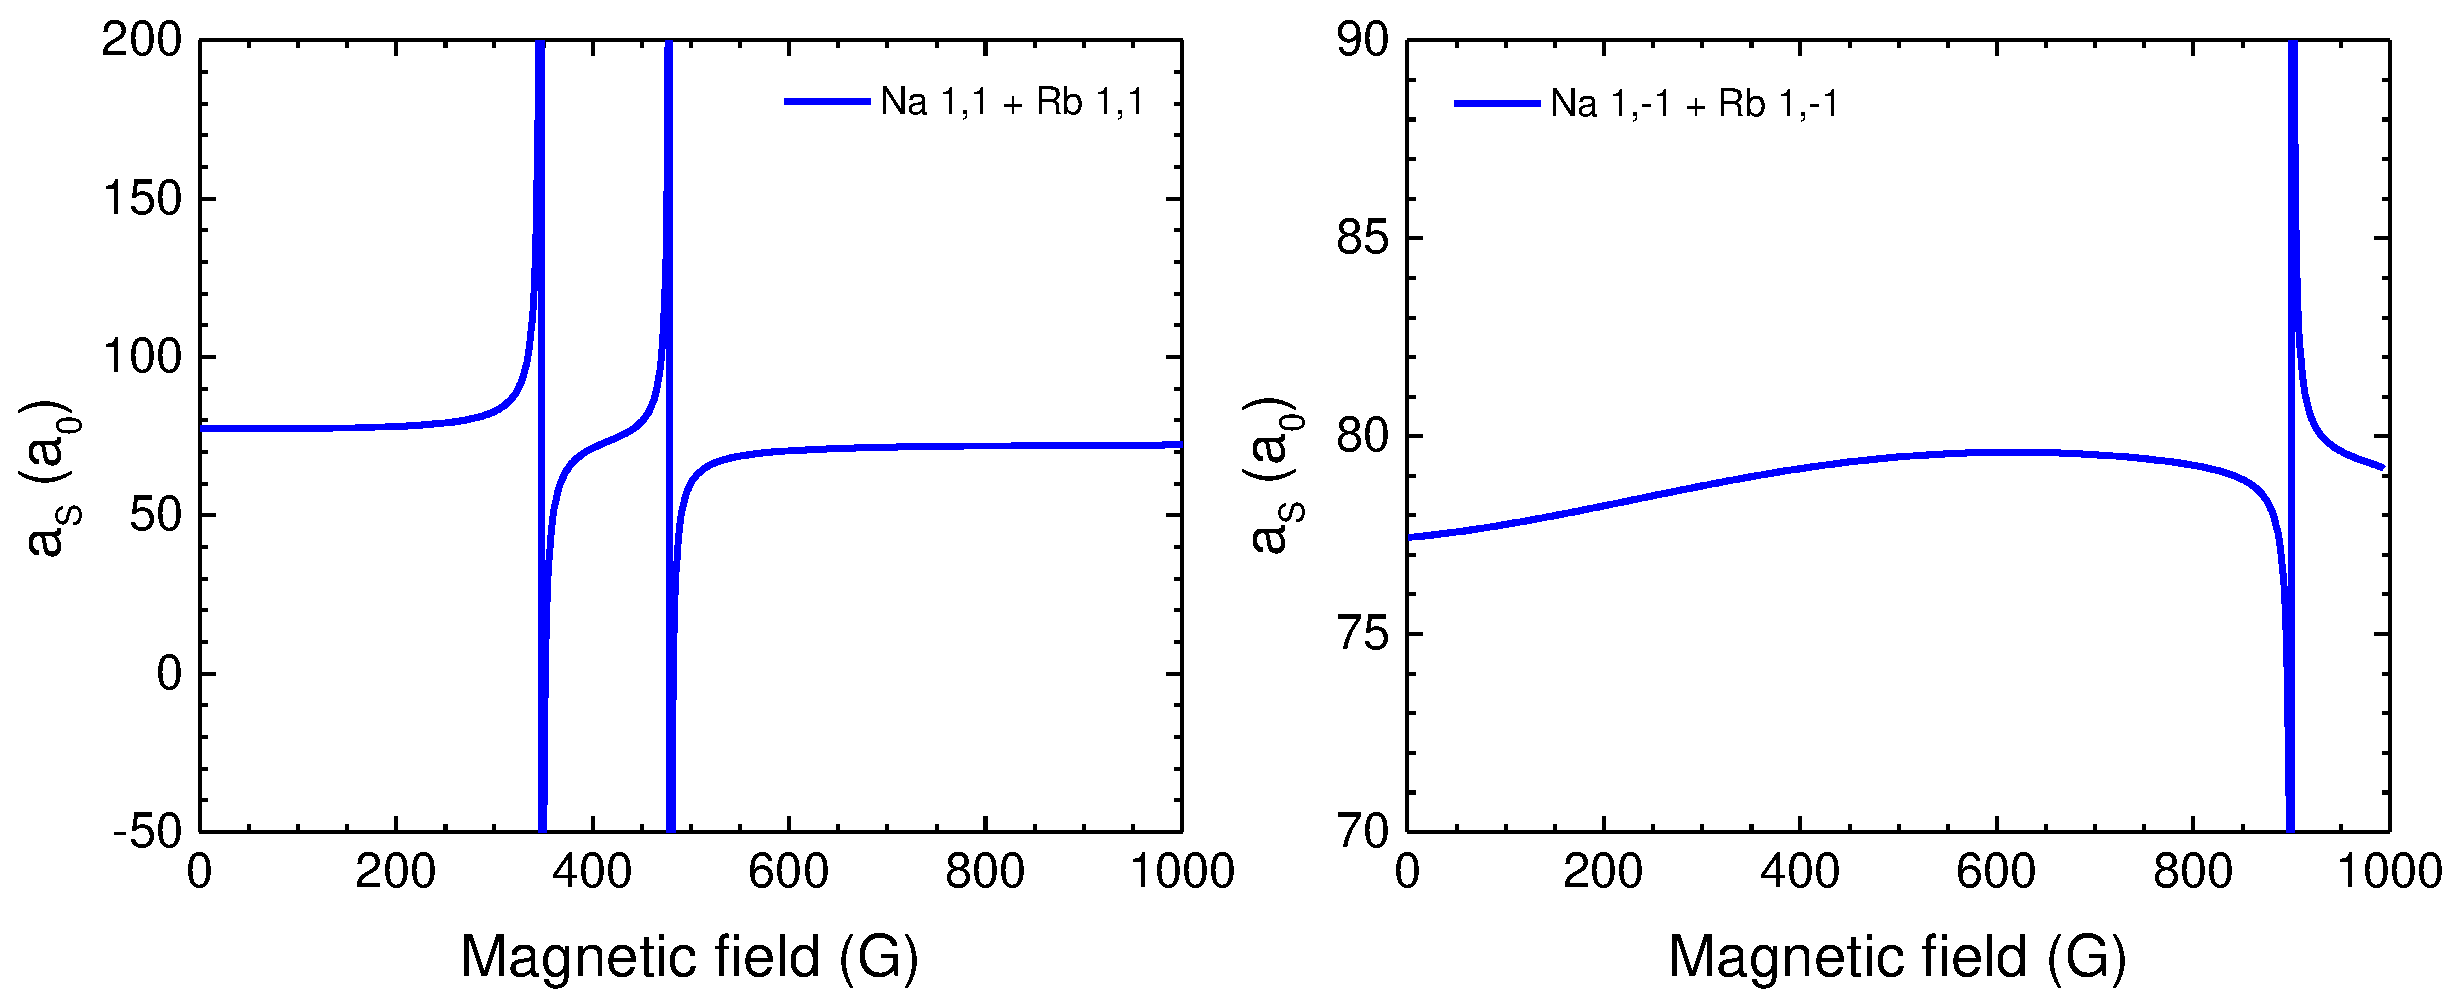
\includegraphics[width = \linewidth]{FR_groupAE.pdf}
\end{center}
\caption[Scattering lengths of Na$\ket{1}$+Rb$\ket{1}$ and Na$\ket{-1}$+Rb$\ket{-1}$ elastic channels]{Both Na$\ket{1}$+Rb$\ket{1}$ and Na$\ket{-1}$+Rb$\ket{-1}$ are elastic channels. Here we only plot the real part of the scattering length since there is no imaginary part. Two resonances show in Na$\ket{1}$+Rb$\ket{1}$ channel and one in Na$\ket{-1}$+Rb$\ket{-1}$ channel. A smooth variation of the scattering length is obvious in Na$\ket{-1}$+Rb$\ket{-1}$ channel.}
\label{FR_groupAE}
\end{figure}

% about elastic channel (done 2021-8-23 14:57:59)
As shown in Table~\ref{fst} and in Fig. \ref{FR_groupAE}, Na$\ket{1}$+Rb$\ket{1}$ Na$\ket{-1}$+Rb$\ket{-1}$ are two channels with all resonances elastic, which means there is no possible for the scattering to other channels. These resonances are a pole as shown in the scattering length plot following the $1/(B-B_0)$ variation. If only considering the two-body collision, one would not have the loss peak as shown in Fig. \ref{FR_loss} or Fig. \ref{FR_more}, because increasing the scattering length only means increasing the elastic collision rate. So, the loss peaks in those measurements are the result of the three-body loss.

% group B for total M=1 (done 2021-8-23 14:51:43)
\begin{figure}[htb]
\begin{center}
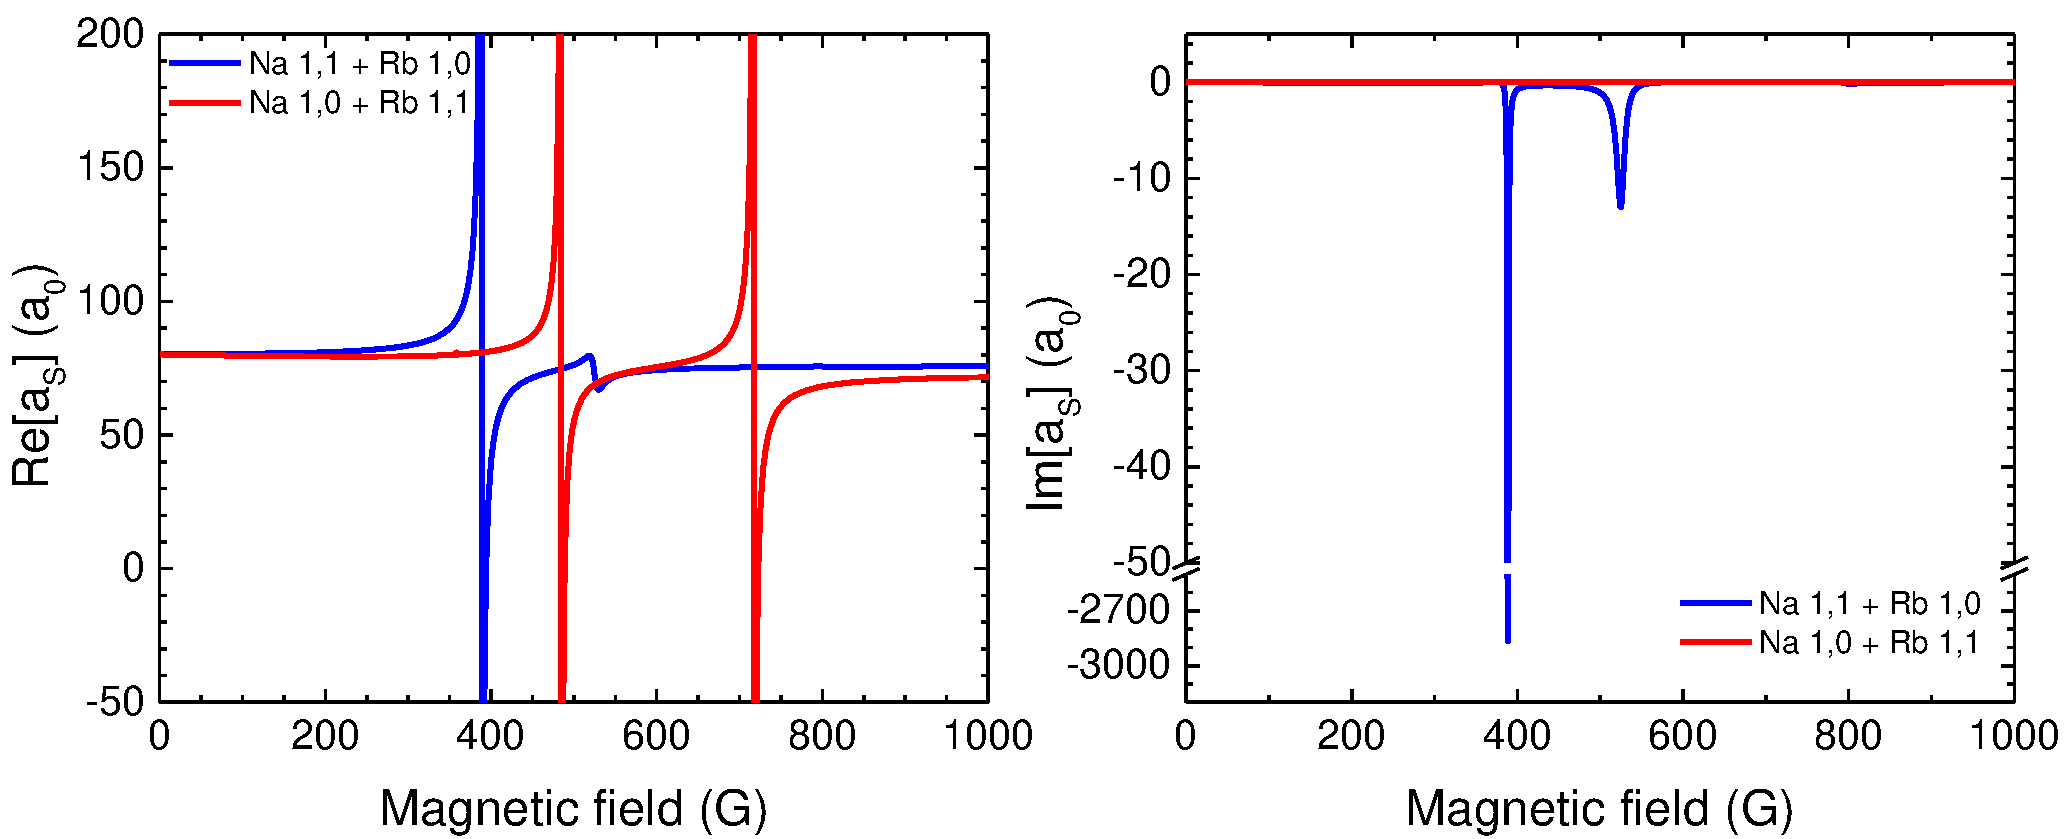
\includegraphics[width = \linewidth]{FR_groupB.pdf}
\end{center}
\caption[Scattering lengths of $M_F=1$ channels]{Scattering lengths of $M_F=1$ channels, including Na$\ket{1}$+Rb$\ket{0}$ and Na$\ket{0}$+Rb$\ket{1}$. Left(right) shows the real(imaginary) part of the scattering length. For Na$\ket{1}$+Rb$\ket{0}$ channel there are two inelastic resonance with non-zero imaginary part of scattering length.}
\label{FR_groupB}
\end{figure}
% group C for total M=0 (done 2021年8月24日12:12:39)
\begin{figure}[htb]
\begin{center}
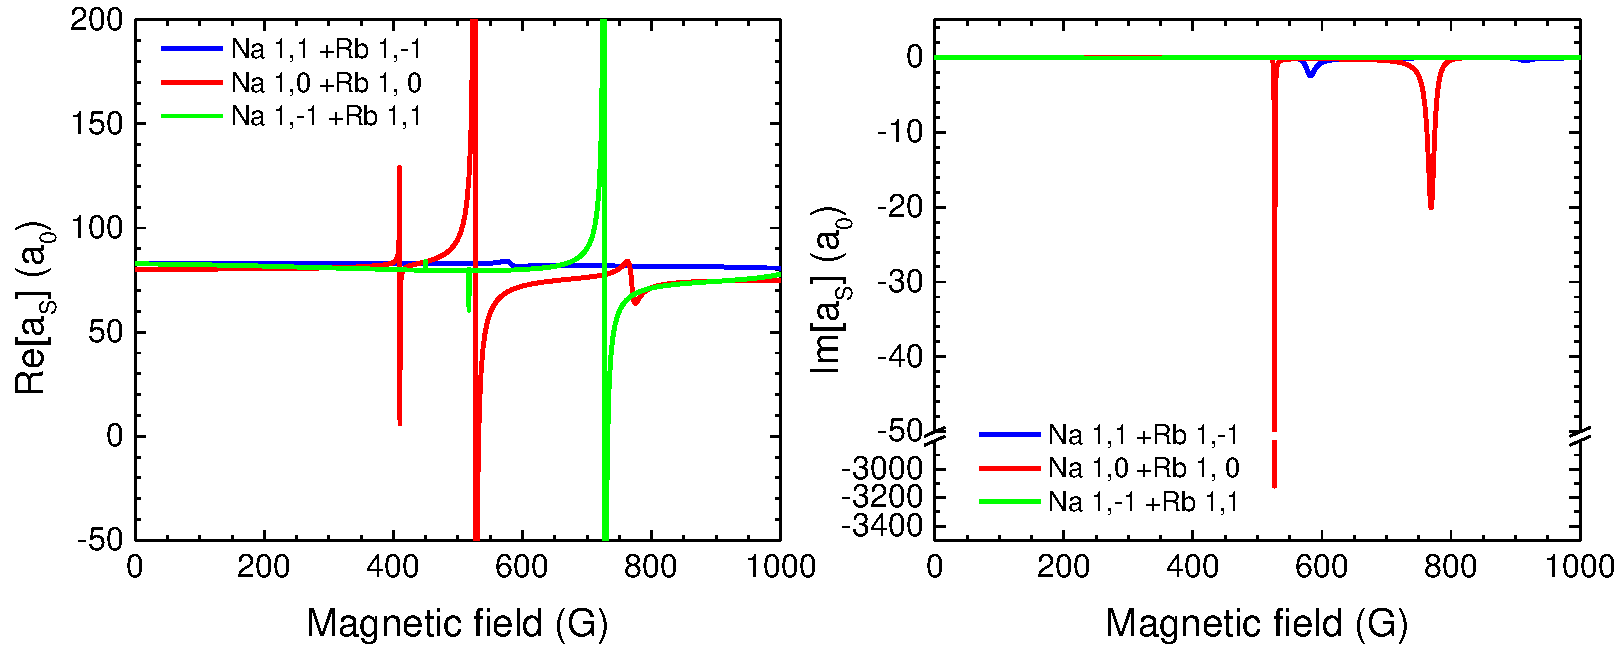
\includegraphics[width = \linewidth]{FR_groupC.pdf}
\end{center}
\caption[Scattering lengths of $M_F=0$ channels]{Scattering lengths of $M_F=0$ channels, including Na$\ket{1}$+Rb$\ket{-1}$, Na$\ket{0}$+Rb$\ket{0}$ and Na$\ket{-1}$+Rb$\ket{1}$. Left(right) shows the real(imaginary) part of the scattering length.}
\label{FR_groupC}
\end{figure}

% about inelastic channel I (done 2021年8月24日12:08:25)
When an inelastic channel is present, the states at the threshold are quasi-bound, so using FIELD is more complicated. Instead, the FRs are located by computing the scattering lengths for magnetic fields up to 1000 G using the MOLSCAT program~\cite{molscat:2019,mbf-github:2020}. Once an FR is located, the resonance parameters are then determined following the regularized scattering length or fully complex procedure of Ref.~\cite{Frye2017}. In this case, the scattering length is complex and shows an oscillation rather than a pole at resonance \cite{Hutson:res:2007}. Such a resonance is termed decayed, and the procedure generates the resonant scattering length $a_{\rm res}$ and the inelastic width $\Gamma_{\rm inel}$ in addition to $B_0^{\rm cc}$, $\Delta$ and $a_{\rm bg}$.

% about inelastic channel II (done 2021年8月24日12:09:06)
The calculation reproduces all the observed $s$-wave resonances. As shown in Table~\ref{fst}, the deviations between $B_0^{\rm cc}$ and $B_0^{\rm exp}$ are within 0.5 G for most of the elastic FRs, labelled by ``N'' in the last column ``inel?''. The only exception is the resonance observed at 410.9 G for the entrance channel $\ket{0} + \ket{0}$, for which $B_0^{\rm cc}$ is 1.1 G lower. As shown in Fig.~\ref{FR_Zeeman-BC}(b), this channel features a nearby switchover between the relative channel energies near 450 G. The four $s$-wave resonances for the entrance channels $\ket{1}+\ket{1}$ and $\ket{0}+ \ket{1}$ all have calculated resonance widths $\Delta$ of several Gauss. They should all be useful for investigating \Na--\Rb mixtures with tunable interactions. These resonances also have rather small calculated effective ranges, on the order of 10s of $a_0$; thus, using the scattering lengths should be sufficient for most applications.

% Zeeman energy for $M_F=1$ and $M_F=0$ channels (done 2021-8-23 10:26:28)
\begin{figure}[htb]
\begin{center}
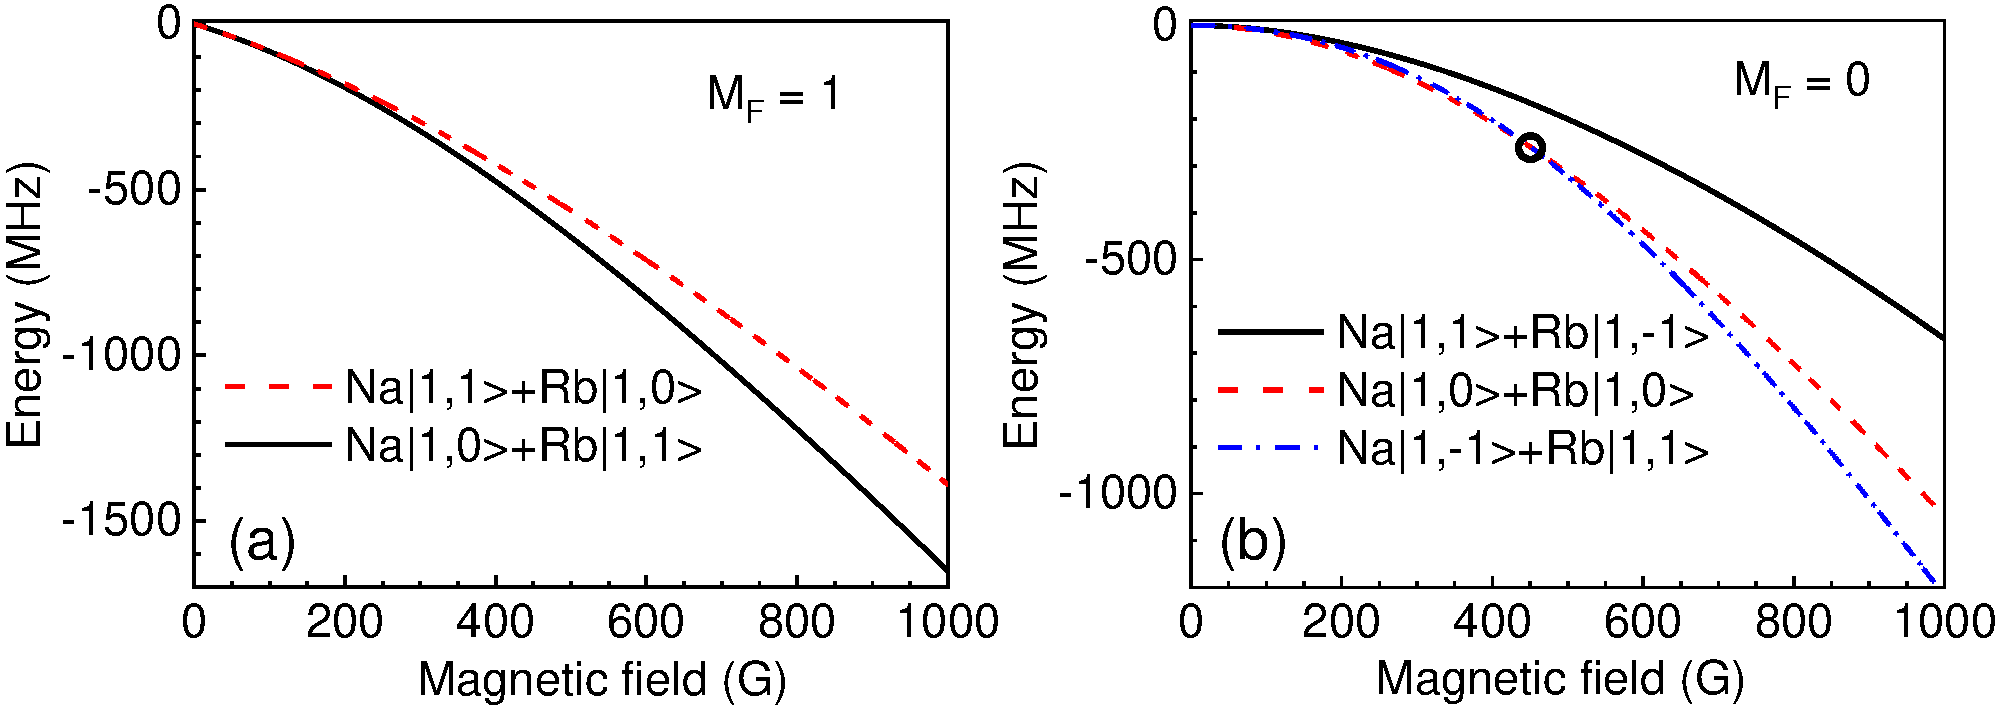
\includegraphics[width = \linewidth]{FR_Zeeman-BC.pdf}
\end{center}
\caption[Zeeman energy for $M_F=1$ and $M_F=0$ channels]{(a) Channel energies for the manifold with $M_F = 1$ for magnetic field up to 1000 G. (b) The same for the manifold with $M_F = 0$. The energies of the channels $\ket{0}+\ket{0}$ and $\ket{-1}+\ket{1}$ cross each other near 450 G, as marked by the black open circle. For each $M_F$, atom pairs in higher-energy channels can undergo inelastic loss by spin exchange to the lower-energy channels.}
\label{FR_Zeeman-BC}
\end{figure}

% about inelastic channel III (done 2021-8-24 12:09:25)
The decayed FRs can have very different characters, depending on $a_\textrm{res}$ and/or $\Gamma_\textrm{inel}$. When $a_\textrm{res}$ is large and $\Gamma_\textrm{inel}\ll\Delta$, the resonance \emph{may} be fairly similar to the elastic case and be dominated by three-body loss. However, when $a_\textrm{res}$ is small and $\Gamma_\textrm{inel}$ is comparable to or larger than $\Delta$, the loss is more likely to be dominated by two-body loss. This looks to be the case for the resonances at 522 G for $\ket{1}+\ket{0}$, at 759 G for $\ket{0}+\ket{0}$, and the unobserved one at 420 G for $\ket{-1}+\ket{1}$. It is also true for both resonances for $\ket{1}+\ket{-1}$, but for those there is a significant \emph{background} loss characterized by the imaginary part of $a_\textrm{bg}$.

% group D for total M=-1 (done 2021年8月24日12:12:28)
\begin{figure}[htb]
\begin{center}
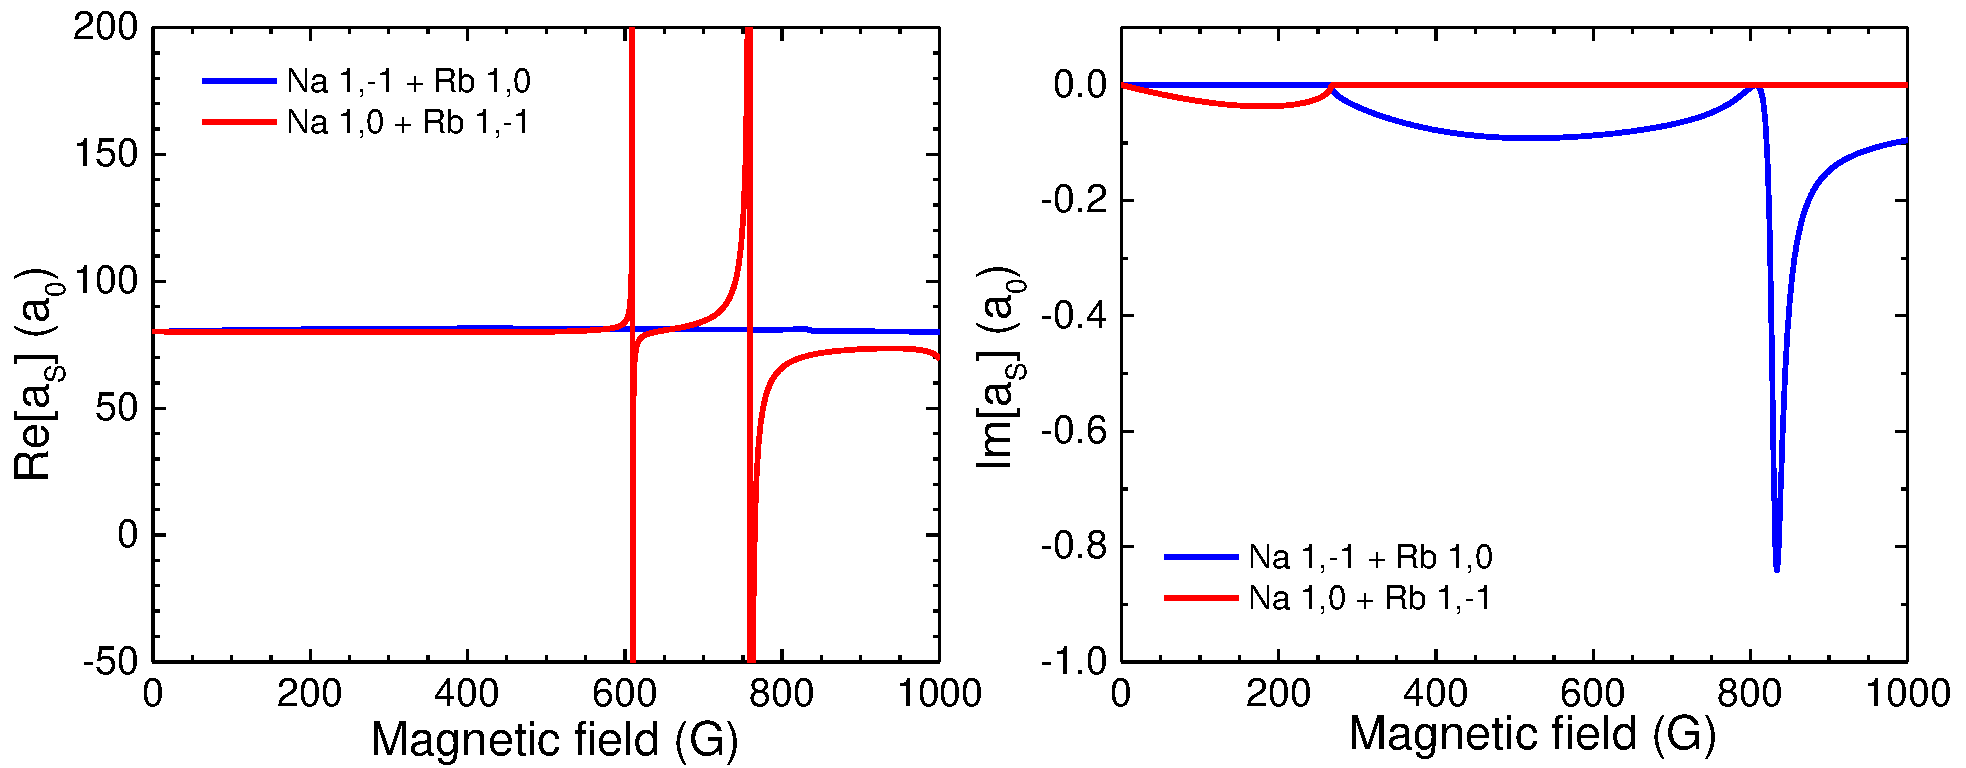
\includegraphics[width = \linewidth]{FR_groupD.pdf}
\end{center}
\caption[Scattering lengths of $M_F=-1$ channels]{Scattering lengths of $M_F=-1$ channels, including Na$\ket{0}$+Rb$\ket{-1}$ and Na$\ket{-1}$+Rb$\ket{0}$. Left(right) shows the real(imaginary) part of the scattering length.}
\label{FR_groupD}
\end{figure}

% about inelastic channel IV
For the decayed resonances with $\Gamma_\textrm{inel} <1$ at 388 G for $\ket{1}+\ket{0}$ and at 526 G for $\ket{0}+\ket{0}$, the calculated resonance positions $B_0^{\rm cc}$ agree with the measured resonance positions $B_0^{\rm exp}$ very well. However, deviations up to several Gauss are observed for inelastic resonances with large $\Gamma_\textrm{inel}$. These can be attributed to several factors. For the two resonances with very broad observed loss spectra at 522 G for $\ket{1}+\ket{0}$ and at 759 G for $\ket{0}+\ket{0}$, the resonance centers have large uncertainties near 10 G. In addition, in presence of the background loss, the two-body loss induced by these resonances has an asymmetric (Fano-like) profile and its measured peak is not at $B_0$. Finally, although we have not studied them carefully, some nearby intraspecies FRs in Na or Rb may also affect the measurements of the resonance positions.

% about those not observed
Several resonances predicted by the coupled-channel calculation are not observed experimentally. Most of these are very narrow ones with calculated $\Delta$ in the mG range. No resonance is found from the calculation for the entrance channel $\ket{0}+\ket{-1}$. In addition, we have not searched experimentally for FRs in the entrance channel $\ket{-1}+\ket{0}$ although the calculation indicates that two resonances should exist.

% about p-wave resonances and some comments
Table~\ref{fst} also lists the several $p$-wave FRs observed by~\cite{Wang2013} for the entrance channels $\ket{1}+\ket{1}$ and $\ket{-1}+\ket{-1}$. As mentioned above, we have not attempted to improve the agreement between the current calculation and the experiment by including the dependence of the atomic hyperfine coupling on $R$. We note that Ref.~\cite{Cui2018}, which presented a compilation of FRs for alkali atoms calculated with multichannel quantum defect theory (MQDT), identified the resonance near 284 G as a ``broad'' $p$-wave resonance. It would be possible to perform a full-scale coupled-channel fitting to these resonances. This, however, is not pursued here as it would involve further adjustments to the potential parameters, beyond those used in Ref.\cite{guo2021leehuangyang}. In view of the inaccuracy of the loss spectroscopy compared with the measurements of FM binding energies, we believe such fitting is not currently justified.

\subsection{Na-Na and Rb-Rb scattering length}

% calculation
Besides interspecies Na-Rb scattering properties, we also study the intraspecies scattering length for Na-Na and Rb-Rb, because the droplet experiment needs all three scattering lengths. Out calculation directly send the potential file from \cite{} to MOLSCAT \cite{} and then use the molscat modular to obtain the scattering length. The Feshbach resonances for Na-Na and Rb-Rb are all far away from 347 G, where we study the droplet \cite{}. However, Na-Na scattering length varies with magnetic field very smoothly, even without resonance. As shown in Fig. \ref{FR_NaNa}, From 0 to around 800 G, we have a scattering length changing from 54.5 $a_0$ to about 64 $a_0$. For magnetic field around 350 G, i.e. the field for forming droplet sample, the scattering length for Na-Na is 60.05 $a_0$. This value is about 10\% larger than in a low magnetic field. 

% Na-Na 1,1 scattering length (done 2021-8-23 14:44:27)
\begin{figure}[htb]
\begin{center}
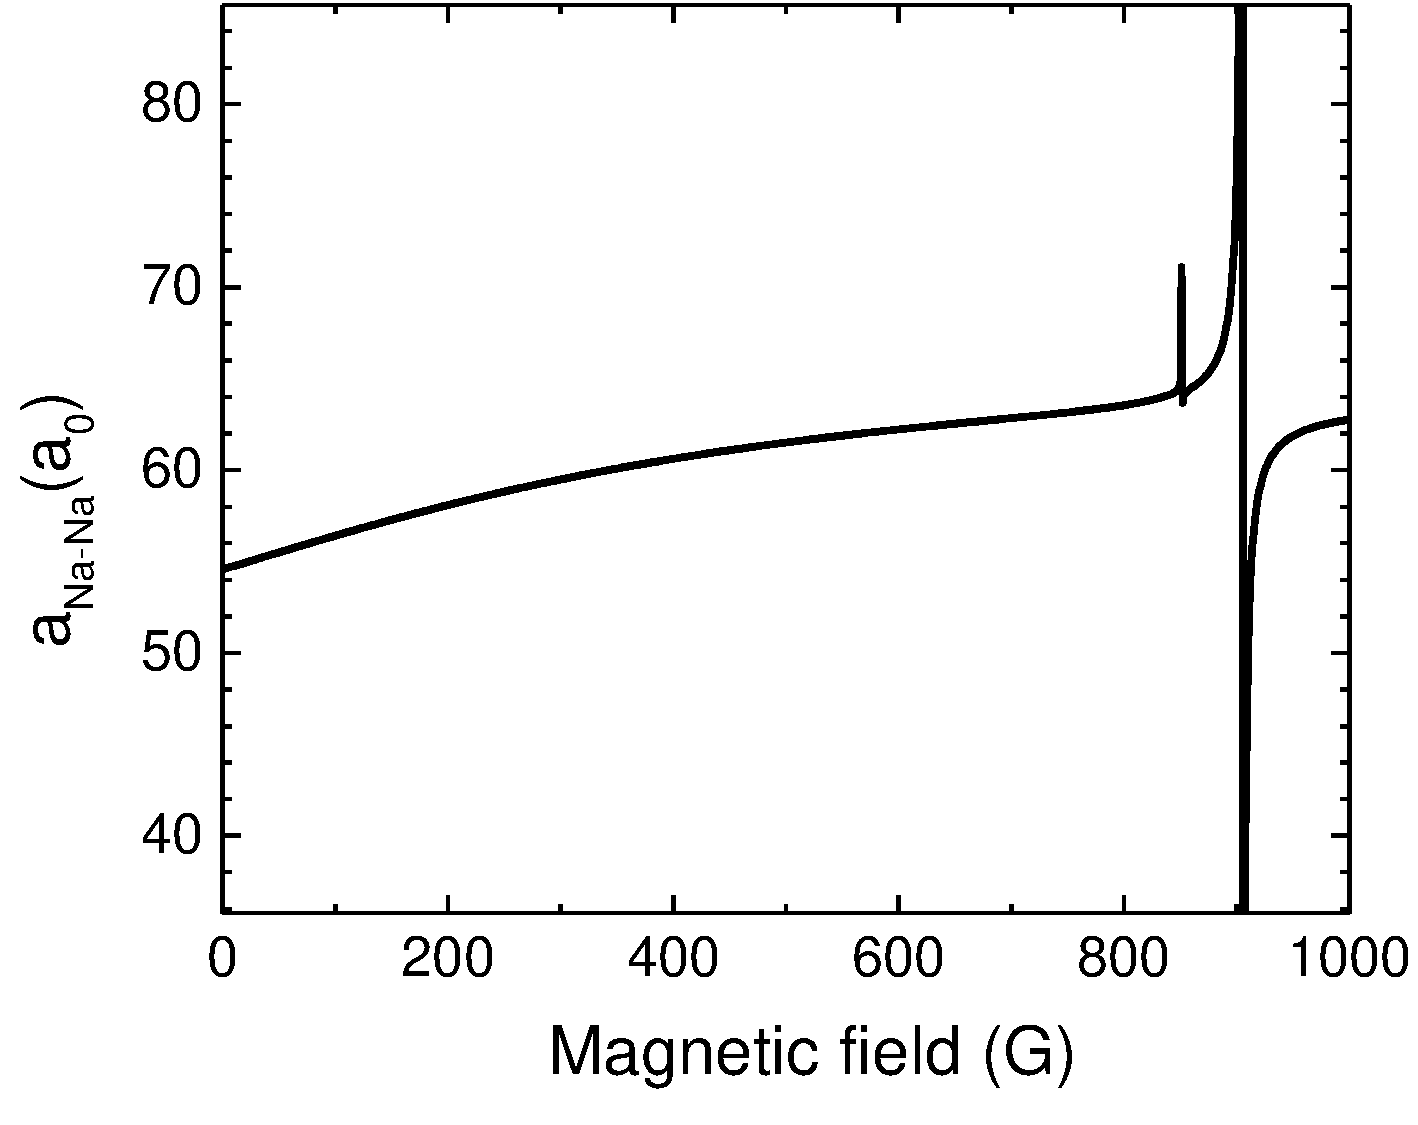
\includegraphics[width = 0.7\linewidth]{FR_NaNa.pdf}
\end{center}
\caption[Na$\ket{1,1}$ + Na$\ket{1,1}$ scattering length as a function of magnetic field]{Na$\ket{1,1}$ + Na$\ket{1,1}$ scattering length as a function of magnetic field. A smooth changing from }
\label{FR_NaNa}
\end{figure}

% more comments
Verifying the Na-Na scattering length value is not easy since the smooth-changing background scattering length only has about 10\% to 20\% variation. Typical methods for measuring $s$-wave scattering length, such as measurement of elastic collision rate by tracing the thermalization process\cite{} or by measuring the BEC expansion\cite{}, are all difficult and need precisely calibration of some other physical parameter (such as atomic number in the second method). These measurements are prone to have an error with 10\% to 20\%. On the other hand, the coupled-channel calculation is the most precise method and is an ab initio calculation that offers reliable numbers. So, we directly take the calculated one.